% defer/rcuusage.tex
% mainfile: ../perfbook.tex
% SPDX-License-Identifier: CC-BY-SA-3.0

\subsection{RCU Usage}
\label{sec:defer:RCU Usage}
\OriginallyPublished{Section}{sec:defer:RCU Usage}{RCU Usage}{Linux Weekly News}{PaulEMcKenney2008WhatIsRCUUsage}

\begin{table}[tb]
\renewcommand*{\arraystretch}{1.2}
\centering
\small
\begin{tabular}{ll}
\toprule
Mechanism RCU Replaces & Section \\
\midrule
Reader-writer locking &
	Section~\ref{sec:defer:RCU is a Reader-Writer Lock Replacement} \\
Restricted reference-counting mechanism &
	Section~\ref{sec:defer:RCU is a Restricted Reference-Counting Mechanism} \\
Bulk reference-counting mechanism &
	Section~\ref{sec:defer:RCU is a Bulk Reference-Counting Mechanism} \\
Poor man's garbage collector &
	Section~\ref{sec:defer:RCU is a Poor Man's Garbage Collector} \\
Existence Guarantees &
	Section~\ref{sec:defer:RCU Provides Existence Guarantees} \\
Type-Safe Memory &
	Section~\ref{sec:defer:RCU is a Way of Providing Type-Safe Memory} \\
Wait for things to finish &
	Section~\ref{sec:defer:RCU is a Way of Waiting for Things to Finish} \\
\bottomrule
\end{tabular}
\caption{RCU Usage}
\label{tab:defer:RCU Usage}
\end{table}

This section answers the question ``What is RCU?'' from the viewpoint
of the uses to which RCU can be put.
Because RCU is most frequently used to replace some existing mechanism,
we look at it primarily in terms of its relationship to such mechanisms,
as listed in Table~\ref{tab:defer:RCU Usage}.
Following the sections listed in this table,
Section~\ref{sec:defer:RCU Usage Summary} provides a summary.

\subsubsection{RCU for Pre-BSD Routing}
\label{sec:defer:RCU for Pre-BSD Routing}

Listings~\ref{lst:defer:RCU Pre-BSD Routing Table Lookup}
and~\ref{lst:defer:RCU Pre-BSD Routing Table Add/Delete}
show code for an RCU-protected Pre-BSD routing table
(\path{route_rcu.c}).
The former shows data structures and \co{route_lookup()},
and the latter shows \co{route_add()} and \co{route_del()}.

\begin{listing}[tbp]
\input{CodeSamples/defer/route_rcu@lookup.fcv}
\caption{RCU Pre-BSD Routing Table Lookup}
\label{lst:defer:RCU Pre-BSD Routing Table Lookup}
\end{listing}

\begin{listing}[tbp]
\input{CodeSamples/defer/route_rcu@add_del.fcv}
\caption{RCU Pre-BSD Routing Table Add/Delete}
\label{lst:defer:RCU Pre-BSD Routing Table Add/Delete}
\end{listing}

\begin{fcvref}[ln:defer:route_rcu:lookup]
In Listing~\ref{lst:defer:RCU Pre-BSD Routing Table Lookup},
line~\lnref{rh} adds the \co{->rh} field used by RCU reclamation,
line~\lnref{re_freed} adds the \co{->re_freed} use-after-free-check field,
lines~\lnref{lock}, \lnref{unlock1}, and~\lnref{unlock2}
add RCU read-side protection,
and lines~\lnref{chk_freed} and~\lnref{abort} add the use-after-free check.
\end{fcvref}
\begin{fcvref}[ln:defer:route_rcu:add_del]
In Listing~\ref{lst:defer:RCU Pre-BSD Routing Table Add/Delete},
lines~\lnref{add:lock}, \lnref{add:unlock}, \lnref{del:lock},
\lnref{del:unlock1}, and~\lnref{del:unlock2} add update-side locking,
lines~\lnref{add:add_rcu} and~\lnref{del:del_rcu} add RCU update-side protection,
line~\lnref{del:call_rcu} causes \co{route_cb()} to be invoked after
a grace period elapses,
and \clnrefrange{cb:b}{cb:e} define \co{route_cb()}.
This is minimal added code for a working concurrent implementation.
\end{fcvref}

\begin{figure}[tb]
\centering
\resizebox{2.5in}{!}{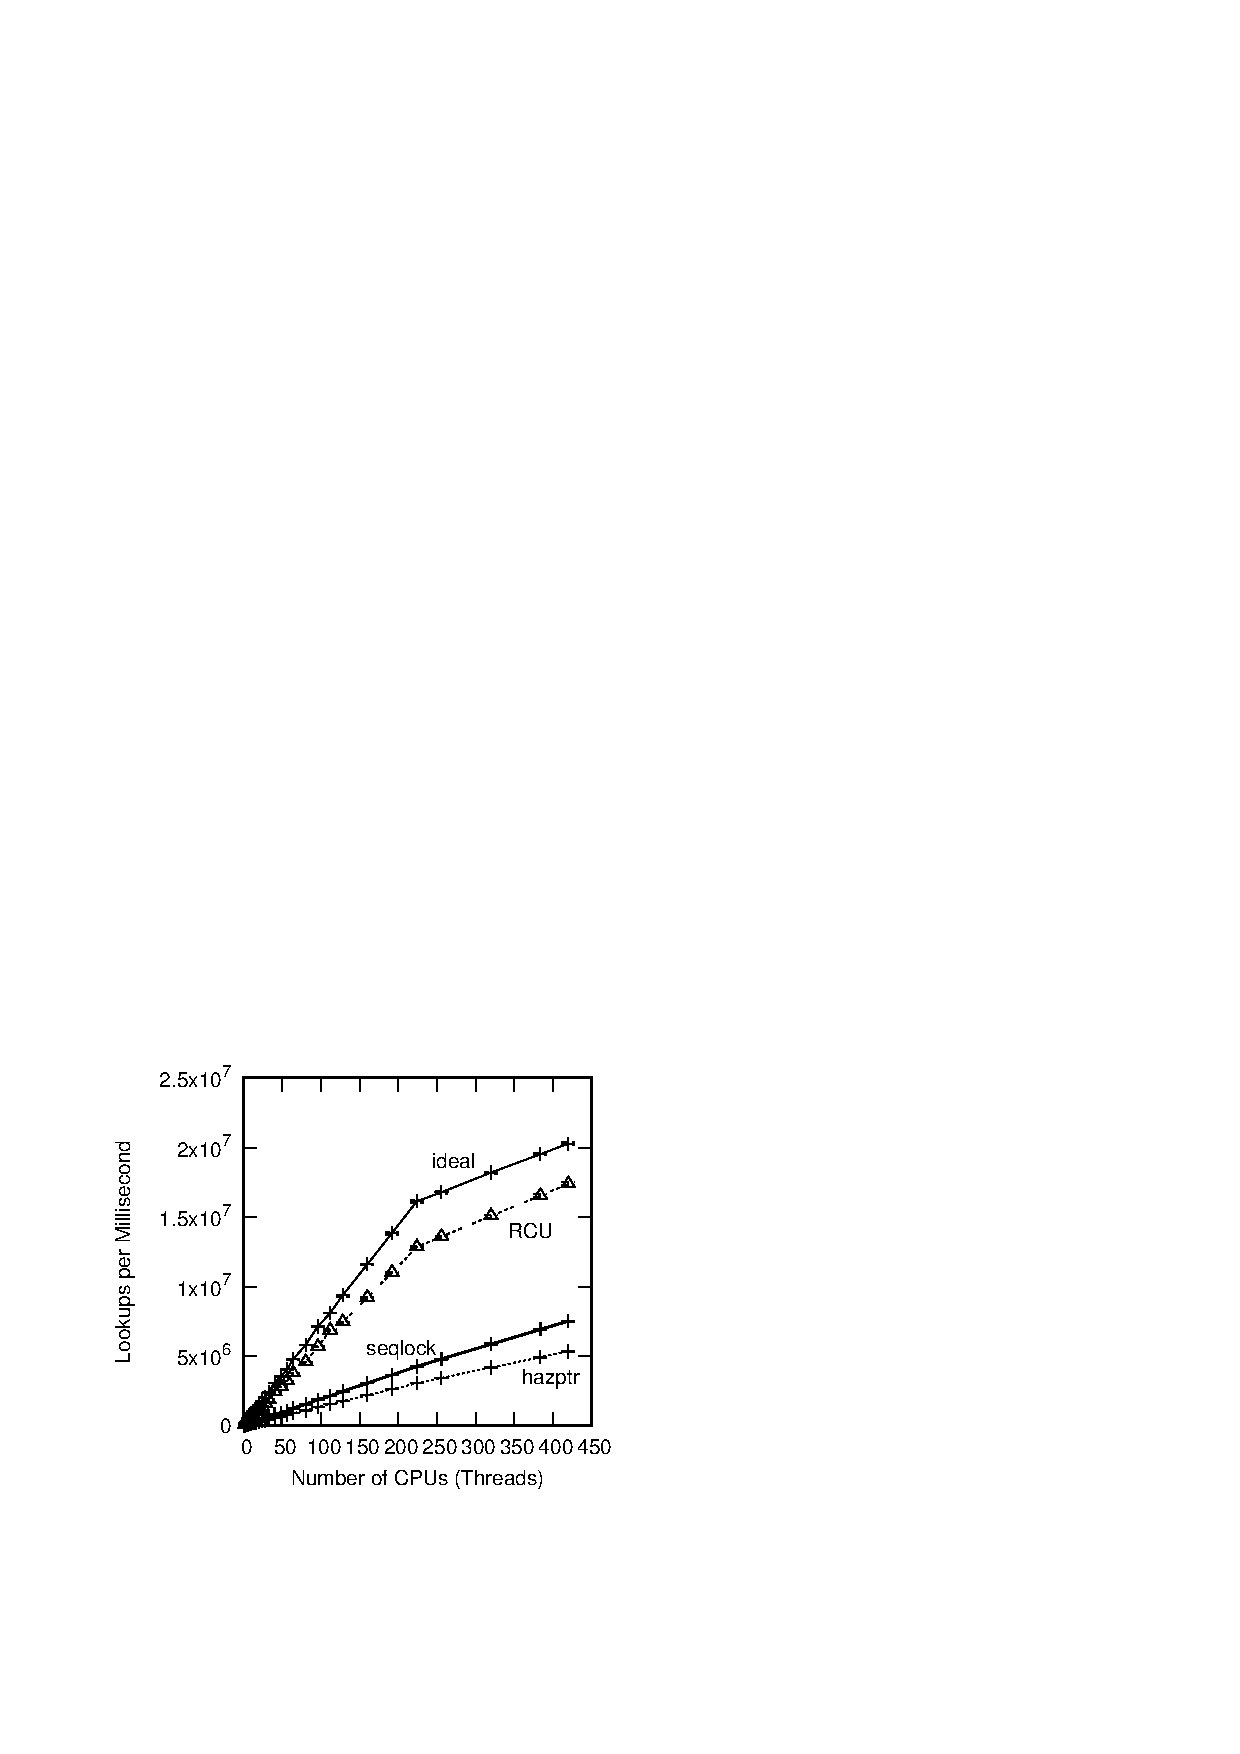
\includegraphics{CodeSamples/defer/perf-rcu}}
\caption{Pre-BSD Routing Table Protected by RCU}
\label{fig:defer:Pre-BSD Routing Table Protected by RCU}
\end{figure}

Figure~\ref{fig:defer:Pre-BSD Routing Table Protected by RCU}
shows the performance on the read-only workload.
RCU scales quite well, and offers nearly ideal performance.
However, this data was generated using the \co{RCU_SIGNAL}
flavor of userspace
RCU~\cite{MathieuDesnoyers2009URCU,PaulMcKenney2013LWNURCU},
for which \co{rcu_read_lock()} and \co{rcu_read_unlock()}
generate a small amount of code.
What happens for the QSBR flavor of RCU, which generates no code at all
for \co{rcu_read_lock()} and \co{rcu_read_unlock()}?
(See Section~\ref{sec:defer:Introduction to RCU},
and especially
Figure~\ref{fig:defer:QSBR: Waiting for Pre-Existing Readers},
for a discussion of RCU QSBR.)

The answer to this shown in
Figure~\ref{fig:defer:Pre-BSD Routing Table Protected by RCU QSBR},
which shows that RCU QSBR's performance and scalability actuaally exceeds
that of the ideal synchronization-free workload.

\QuickQuizSeries{%
\QuickQuizB{
	Wait, what???
	How can RCU QSBR possibly be better than ideal?
	Just what rubbish definition of ideal would fail to be the best
	of all possible results???
}\QuickQuizAnswerB{
	This is an excellent question, and the answer is that modern
	CPUs and compilers are extremely complex.
	But before getting into that, it is well worth noting that
	RCU QSBR's performance advantage appears only in the
	one-hardware-thread-per-core regime.
	Once the system is fully loaded, RCU QSBR's performance drops
	back to ideal.

	The RCU variant of the \co{route_lookup()} search loop actually
	has one more x86 instruction than does the sequential version,
	namely the \co{lea} in the sequence
	\co{cmp}, \co{je}, \co{mov}, \co{cmp}, \co{lea}, and \co{jne}.
	This extra instruction is due to the \co{rcu_head} structure
	at the beginning of the RCU variant's \co{route_entry} structure,
	so that, unlike the sequential variant, the RCU variant's
	\co{->re_next.next} pointer has a non-zero offset.
	Back in the 1980s, this additional \co{lea} instruction might
	have reliably resulted in the RCU variant being slower, but we
	are now in the 21\textsuperscript{st} century, and the 1980s
	are long gone.

	But those of you who read
	\cref{sec:cpu:Pipelined CPUs}
	carefully already knew all of this!

	These counter-intuitive results of course means that any
	performance result on modern microprocessors must be subject to
	some skepticism.
	In theory, it really does not make sense to obtain performance
	results that are better than ideal, but it really can happen
	on modern microprocessors.
	Such results can be thought of as similar to the celebrated
	super-linear speedups (see
	Section~\ref{sec:SMPdesign:Beyond Partitioning}
	for one such example), that is, of interest but also of limited
	practical importance.
	Nevertheless, one of the strengths of RCU is that its read-side
	overhead is so low that tiny effects such as this one are visible
	in real performance measurements.

\begin{figure}[tb]
\centering
\resizebox{2.5in}{!}{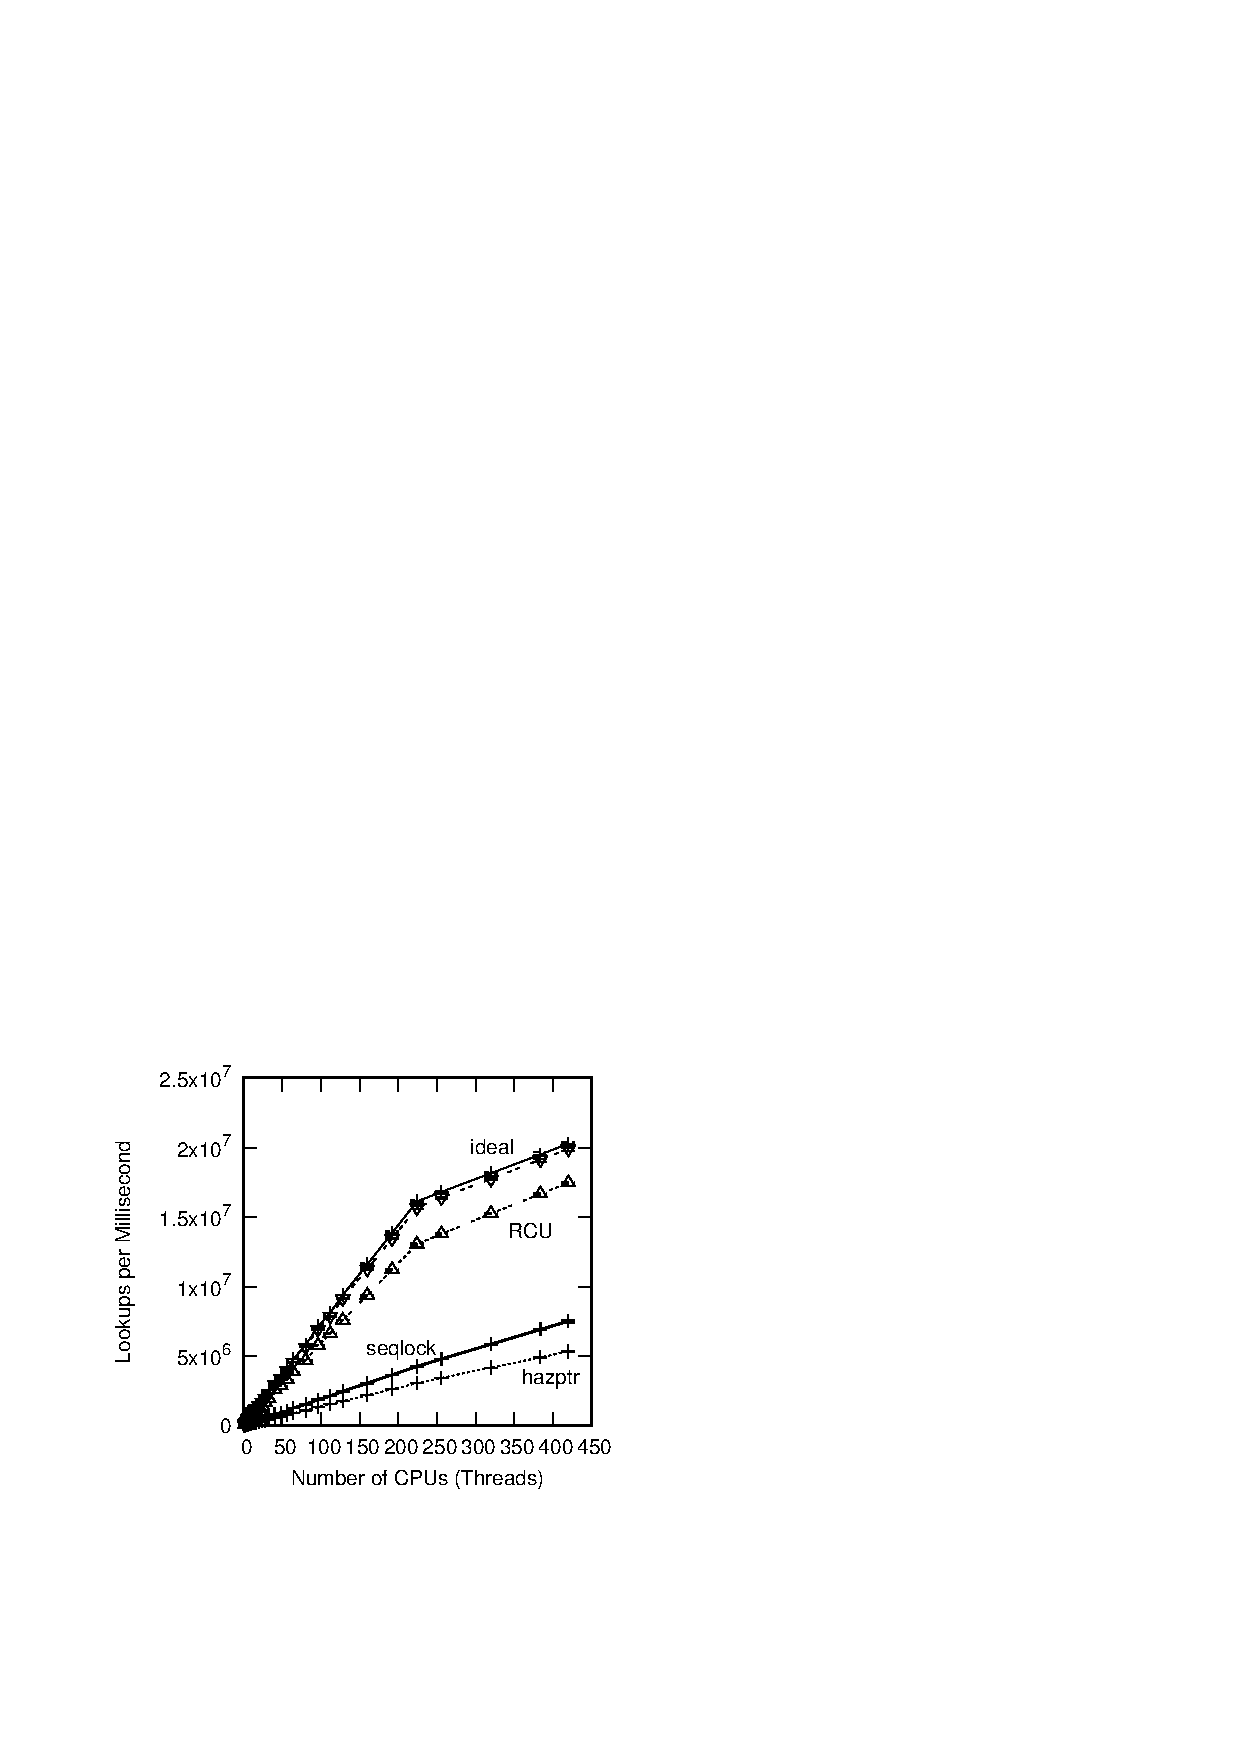
\includegraphics{CodeSamples/defer/perf-rcu-qsbr-qq}}
\caption{Pre-BSD Routing Table Protected by RCU QSBR With Non-Initial \tco{rcu_head}}
\label{fig:defer:Pre-BSD Routing Table Protected by RCU QSBR With Non-Initial rcu-head}
\end{figure}

	This raises the question as to what would happen if the
	\co{rcu_head} structure were to be moved so that RCU's
	\co{->re_next.next} pointer also had zero offset, just the
	same as the sequential variant.
	And the answer, as can be seen in
	Figure~\ref{fig:defer:Pre-BSD Routing Table Protected by RCU QSBR With Non-Initial rcu-head},
	is that this causes RCU QSBR's performance to decrease to where
	it is still very nearly ideal, but no longer super-ideal.
}\QuickQuizEndB
%
\QuickQuizE{
	Given RCU QSBR's read-side performance, why bother with any
	other flavor of userspace RCU?
}\QuickQuizAnswerE{
	Because RCU QSBR places constraints on the overall application
	that might not be tolerable,
	for example, requiring that each and every thread in the
	application regularly pass through a quiescent state.
	Among other things, this means that RCU QSBR is not helpful
	to library writers, who might be better served by other
	flavors of userspace RCU~\cite{PaulMcKenney2013LWNURCU}.
}\QuickQuizEndE
}

\begin{figure}[tb]
\centering
\resizebox{2.5in}{!}{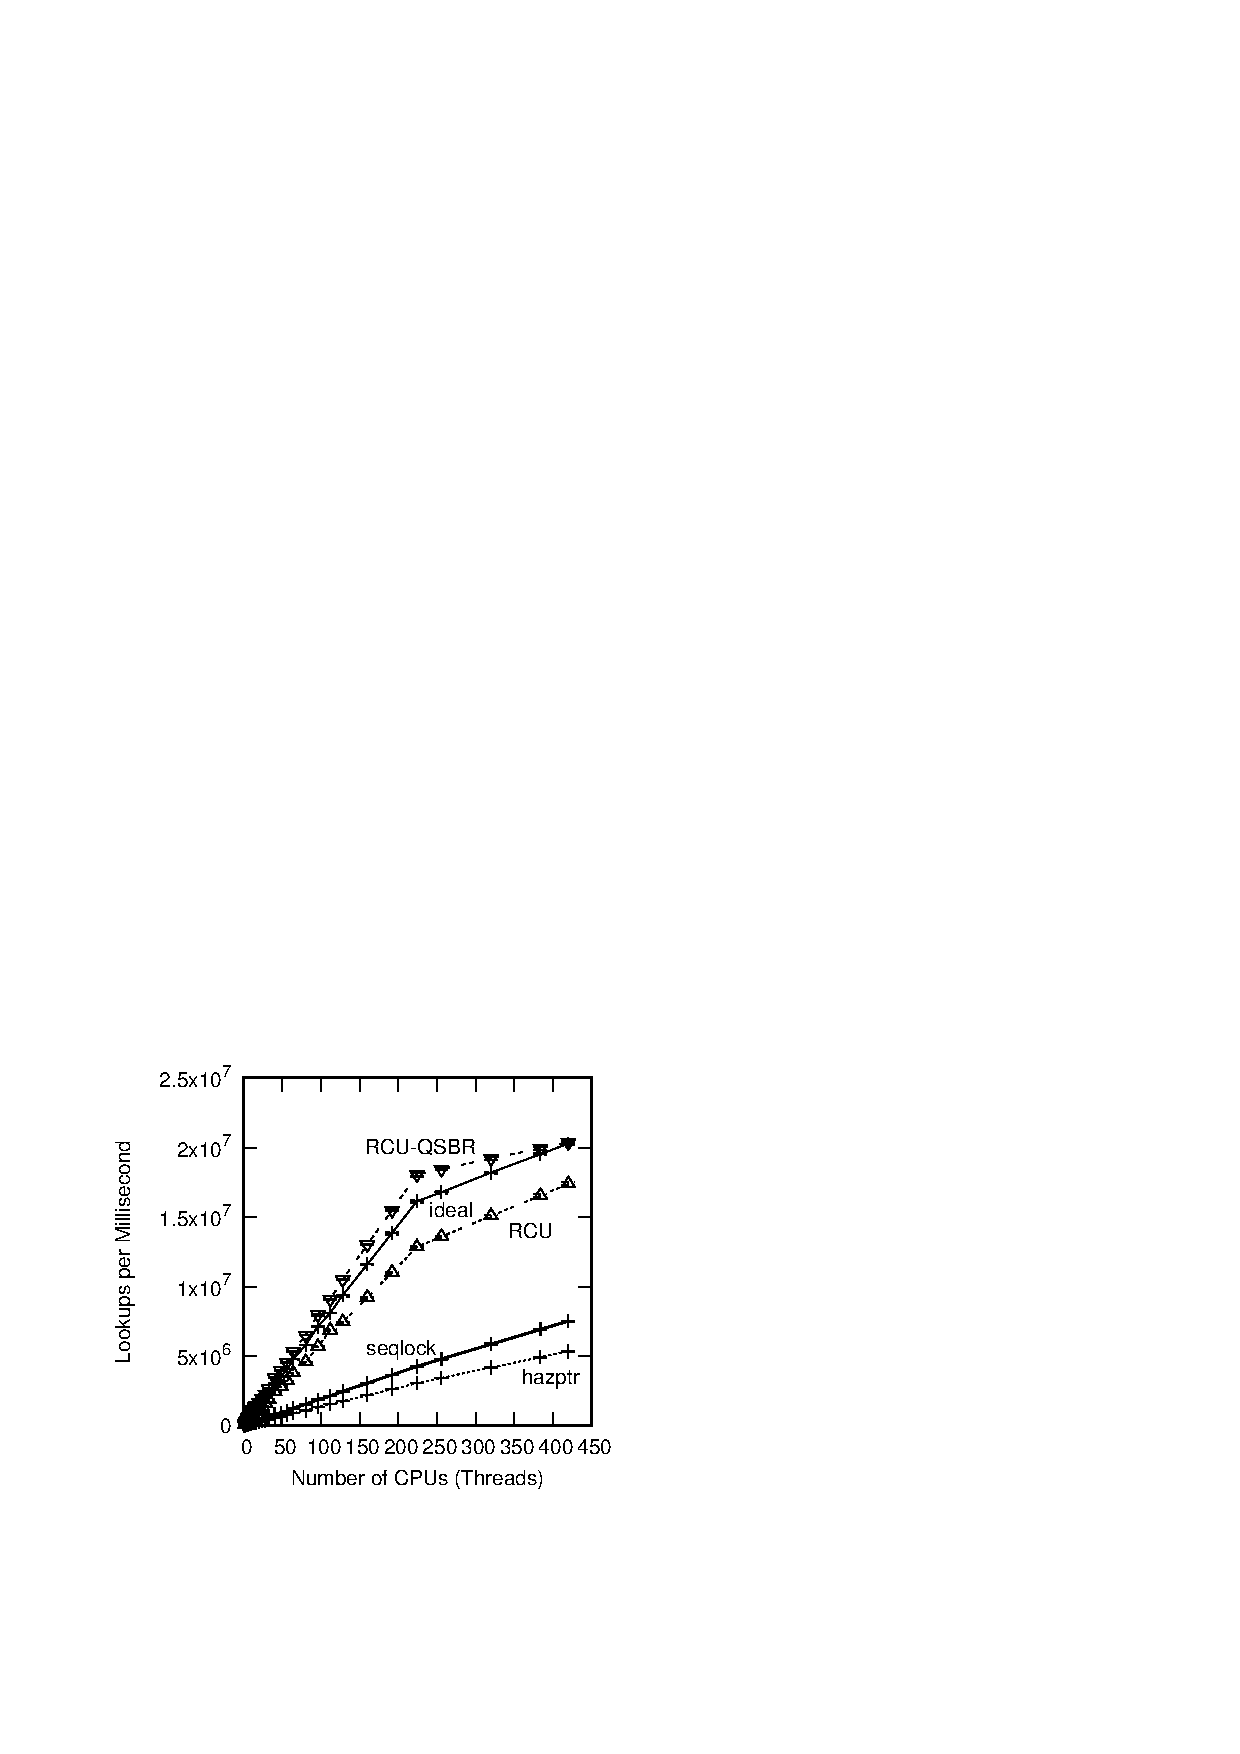
\includegraphics{CodeSamples/defer/perf-rcu-qsbr}}
\caption{Pre-BSD Routing Table Protected by RCU QSBR}
\label{fig:defer:Pre-BSD Routing Table Protected by RCU QSBR}
\end{figure}

\subsubsection{RCU is a Reader-Writer Lock Replacement}
\label{sec:defer:RCU is a Reader-Writer Lock Replacement}

Perhaps the most common use of RCU within the Linux kernel is as
a replacement for reader-writer locking in read-intensive situations.
Nevertheless, this use of RCU was not immediately apparent to me
at the outset, in fact, I chose to implement a lightweight reader-writer
lock~\cite{WilsonCHsieh92a}\footnote{
	Similar to \co{brlock} in the 2.4 Linux kernel and to
	\co{lglock} in more recent Linux kernels.}
before implementing a general-purpose RCU implementation
back in the early 1990s.
Each and every one of the uses I envisioned for the lightweight reader-writer
lock was instead implemented using RCU.
In fact, it was more than
three years before the lightweight reader-writer lock saw its first use.
Boy, did I feel foolish!

The key similarity between RCU and reader-writer locking is that
both have read-side critical sections that can execute in parallel.
In fact, in some cases, it is possible to mechanically substitute RCU API
members for the corresponding reader-writer lock API members.
But first, why bother?

Advantages of RCU include performance,
deadlock immunity, and realtime latency.
There are, of course, limitations to RCU, including the fact that
readers and updaters run concurrently, that low-priority RCU readers
can block high-priority threads waiting for a grace period to elapse,
and that grace-period latencies can extend for many milliseconds.
These advantages and limitations are discussed in the following sections.

\paragraph{Performance}

\begin{figure}[tb]
\centering
\resizebox{2.5in}{!}{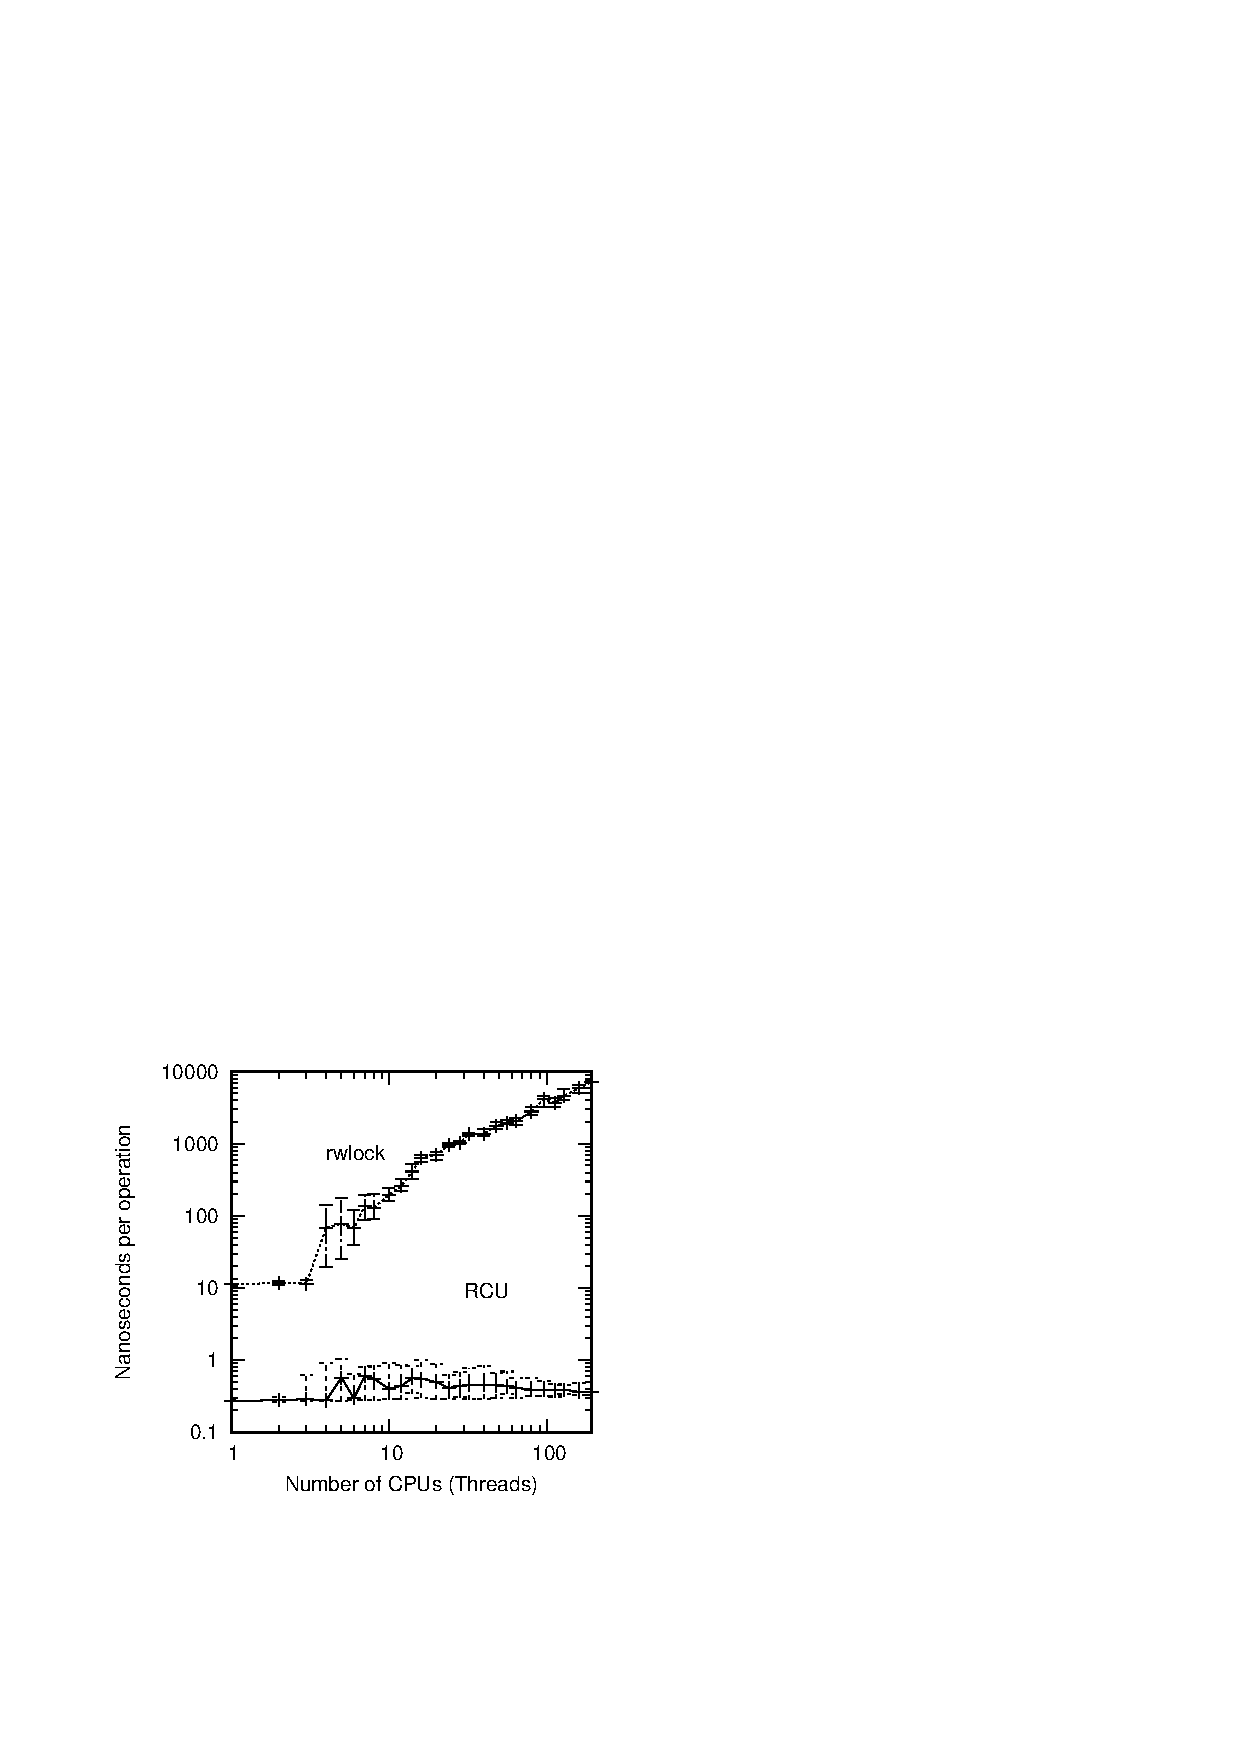
\includegraphics{defer/rwlockRCUperf}}
\caption{Performance Advantage of RCU Over Reader-Writer Locking}
\label{fig:defer:Performance Advantage of RCU Over Reader-Writer Locking}
\end{figure}

The read-side performance advantages of Linux-kernel RCU over
reader-writer locking are shown in
Figure~\ref{fig:defer:Performance Advantage of RCU Over Reader-Writer Locking},
which was generated on a 448-CPU 2.10\,GHz Intel x86 system.

\QuickQuizSeries{%
\QuickQuizB{
	WTF?
	How the heck do you expect me to believe that RCU can have less
	than a 300-picosecond overhead when the clock period at 2.10\,GHz
	is almost 500\,picoseconds?
}\QuickQuizAnswerB{
	First, consider that the inner loop used to
	take this measurement is as follows:

\begin{VerbatimN}
	for (i = nloops; i >= 0; i--) {
		rcu_read_lock();
		rcu_read_unlock();
	}
\end{VerbatimN}

	Next, consider the effective definitions of \co{rcu_read_lock()}
	and \co{rcu_read_unlock()}:

\begin{VerbatimN}
#define rcu_read_lock()   barrier()
#define rcu_read_unlock() barrier()
\end{VerbatimN}

	These definitions constrain compiler code-movement optimizations
	involving memory references, but emit no instructions in and
	of themselves.
	However, if the loop variable is maintained in a register,
	the accesses to \co{i} will not count as memory references.
	Furthermore, the compiler can do loop unrolling,
	allowing the resulting code to ``execute'' multiple passes
	through the loop body simply by incrementing \co{i} by
	some value larger than the value 1.

	So the ``measurement'' of 267 picoseconds is simply the fixed
	overhead of the timing measurements divided by the number of
	passes through the inner loop containing the calls
	to \co{rcu_read_lock()} and \co{rcu_read_unlock()}, plus
	the code to manipulate \co{i} divided by the loop-unrolling
	factor.
	And therefore, this measurement really is in error, in fact,
	it exaggerates the overhead by an arbitrary number of orders
	of magnitude.
	After all, in terms of machine instructions emitted, the actual
	overheads of \co{rcu_read_lock()} and of \co{rcu_read_unlock()}
	are each precisely zero.

	It certainly is not just every day that a timing measurement
	of 267 picoseconds turns out to be an overestimate!
}\QuickQuizEndB

\QuickQuizM{
	Didn't an earlier release of this book show RCU read-side
	overhead way down in the sub-picosecond range?
	What happened???
}\QuickQuizAnswerM{
	Excellent memory!!!
	The overhead in some early releases was in fact roughly
	100~femtoseconds.

	What happened was that RCU usage spread more broadly through the
	Linux kernel, including into code that takes page faults.
	Back at that time, \co{rcu_read_lock()} and \co{rcu_read_unlock()}
	were complete no-ops in \co{CONFIG_PREEMPT=n} kernels.
	Unfortunately, that situation allowed the compiler to reorder
	page-faulting memory accesses into RCU read-side critical
	sections.
	Of course, page faults can block, which destroys those critical
	section.

	Nor was this a theoretical problem:
	A failure actually manifested in 2019.
	Herbert Xu tracked down this failure down and Linus Torvalds
	therefore queued a commit to upgrade \co{rcu_read_lock()} and
	\co{rcu_read_unlock()} to unconditionally include a call to
	\co{barrier()}~\cite{LinusTorvalds2019:RCUreader.barrier}.
	And although \co{barrier()} emits no code, it does constrain
	compiler optimizations.
	And so the price of widespread RCU usage is slightly higher
	\co{rcu_read_lock()} and \co{rcu_read_unlock()} overhead.

	Of course, it is also the case that the older results were obtained
	on a different system than were those shown in
	Figure~\ref{fig:defer:Performance Advantage of RCU Over Reader-Writer Locking}.
	So which change had the most effect, Linus's commit or the change in
	the system?
	This question is left as an exercise to the reader.
}\QuickQuizEndM

\QuickQuizE{
	Why is there such large variation for the \co{rcu} trace in
	Figure~\ref{fig:defer:Performance Advantage of RCU Over Reader-Writer Locking}?
}\QuickQuizAnswerE{
	Keep in mind that this is a log-log plot, so those large-seeming
	\co{rcu} variances in reality span only a few hundred picoseconds.
	And that is such a short time that anything could cause it.
	However, given that the variance decreases with both small and
	large numbers of CPUs, one hypothesis is that the variation is
	due to migrations from one CPU to another.

	Yes, these measurements were taken with interrupts disabled, but
	they were also taken within a guest OS, so that preemption was
	still possible at the hypervisor level.
	Attempting to reduce these variations by running the guest OSes
	at real-time priority (as suggested by Joel Fernandes) is left
	as an exercise for the reader.
}\QuickQuizEndE
}                 % End of \QuickQuizSeries

Note that reader-writer locking is more than an order of magnitude slower
than RCU on a single CPU, and is more than \emph{four} orders of magnitude
slower on 192~CPUs.
In contrast, RCU scales quite well.
In both cases, the error bars cover the full range of the measurements
from 30 runs, with the line being the median.

\begin{figure}[tb]
\centering
\resizebox{2.5in}{!}{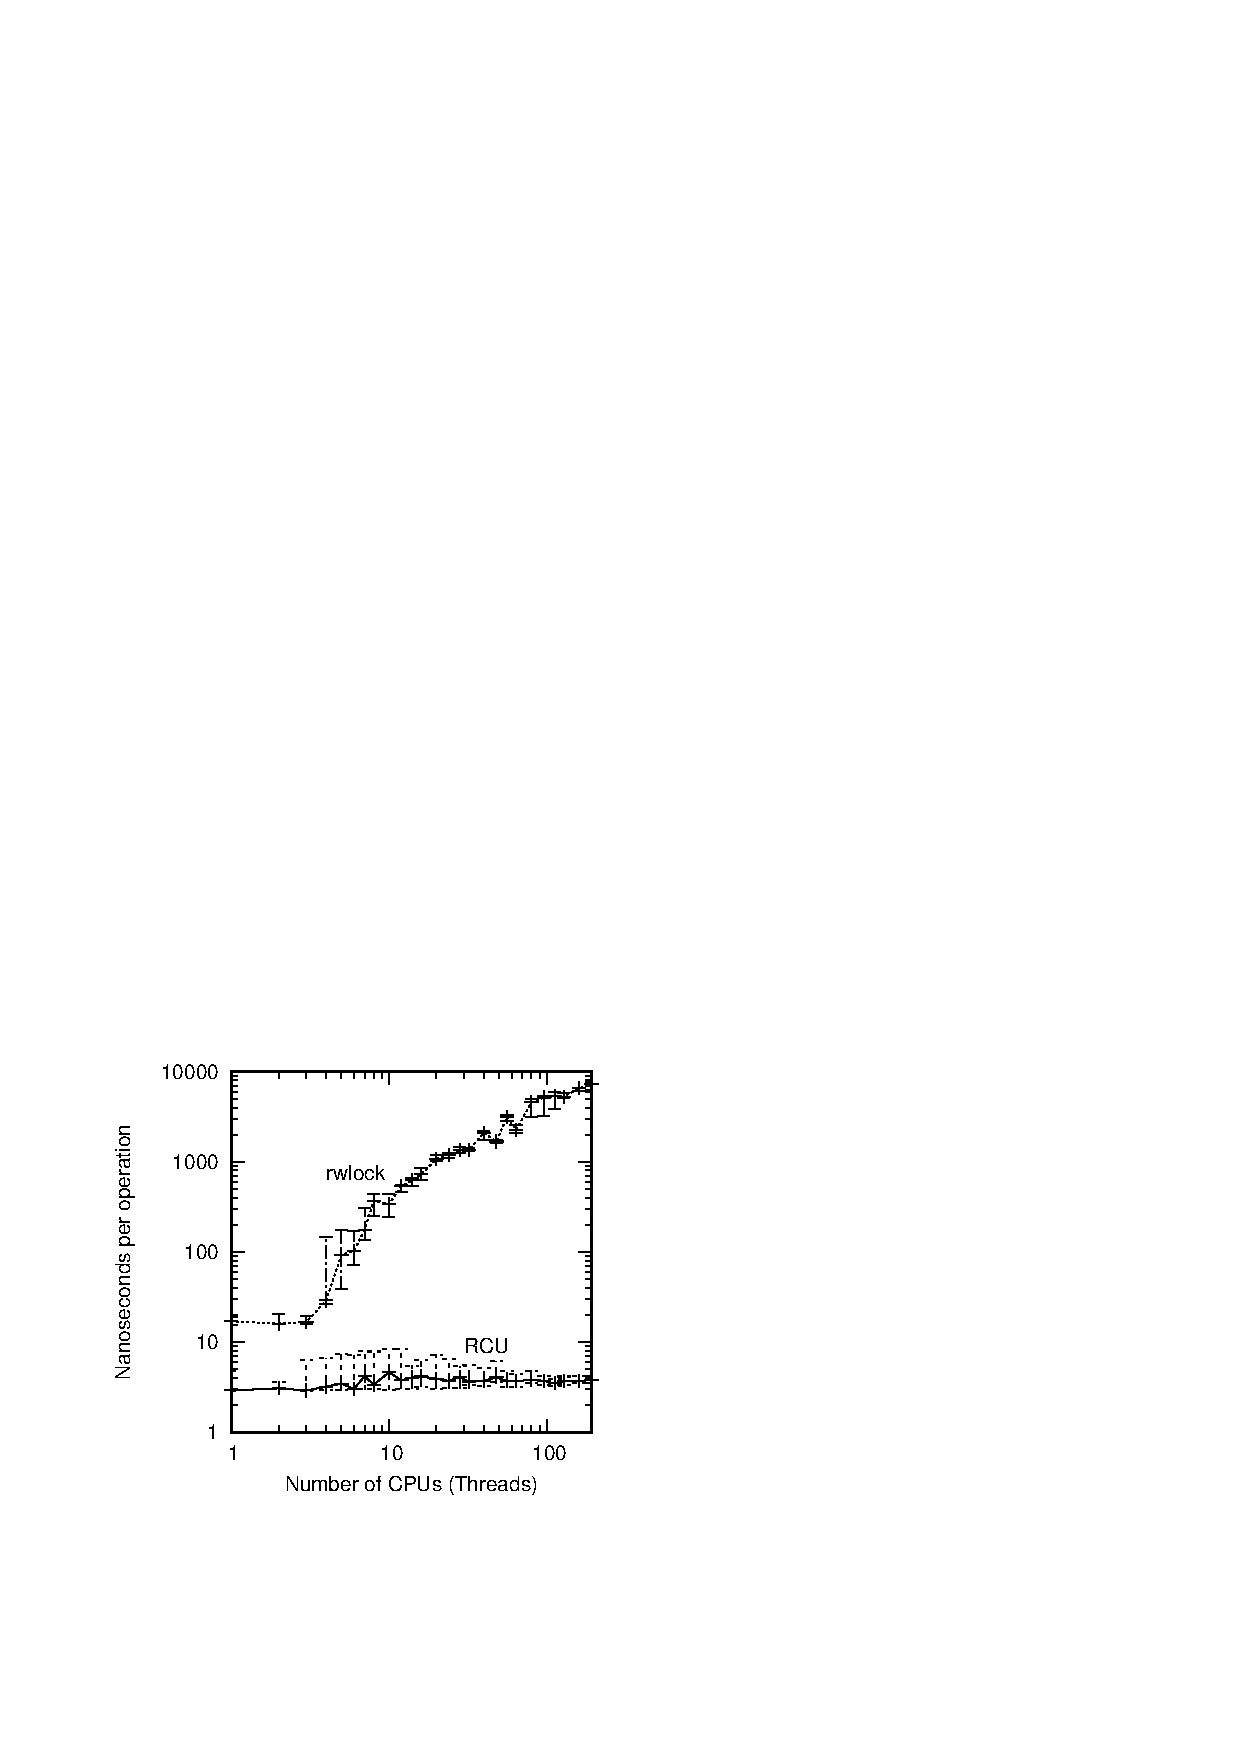
\includegraphics{defer/rwlockRCUperfPREEMPT}}
\caption{Performance Advantage of Preemptible RCU Over Reader-Writer Locking}
\label{fig:defer:Performance Advantage of Preemptible RCU Over Reader-Writer Locking}
\end{figure}

A more moderate view may be obtained from a \co{CONFIG_PREEMPT} kernel,
though RCU still beats reader-writer locking by between a factor of seven
on a single CPU and by three orders of magnitude on 192~CPUs, as shown in
Figure~\ref{fig:defer:Performance Advantage of Preemptible RCU Over Reader-Writer Locking},
which was generated on the same 448-CPU 2.10\,GHz x86 system.
Note the high variability of reader-writer locking at larger numbers of CPUs.
The error bars span the full range of data.

\QuickQuiz{
	Given that the system had no fewer than 448~hardware threads,
	why only 192~CPUs?
}\QuickQuizAnswer{
	Because the script (\path{rcuscale.sh}) that generates this data
	spawn a guest operating system for each set of points gathered,
	and on this particular system, both \co{qemu} and KVM limit the
	number of CPUs that may be configured into a given guest OS.
	Yes, it would have been possible to run a few more CPUs, but
	192 is a nice round number from a binary perspective, given
	that 256 is infeasible.
}\QuickQuizEnd

\begin{figure}[tb]
\centering
\resizebox{2.5in}{!}{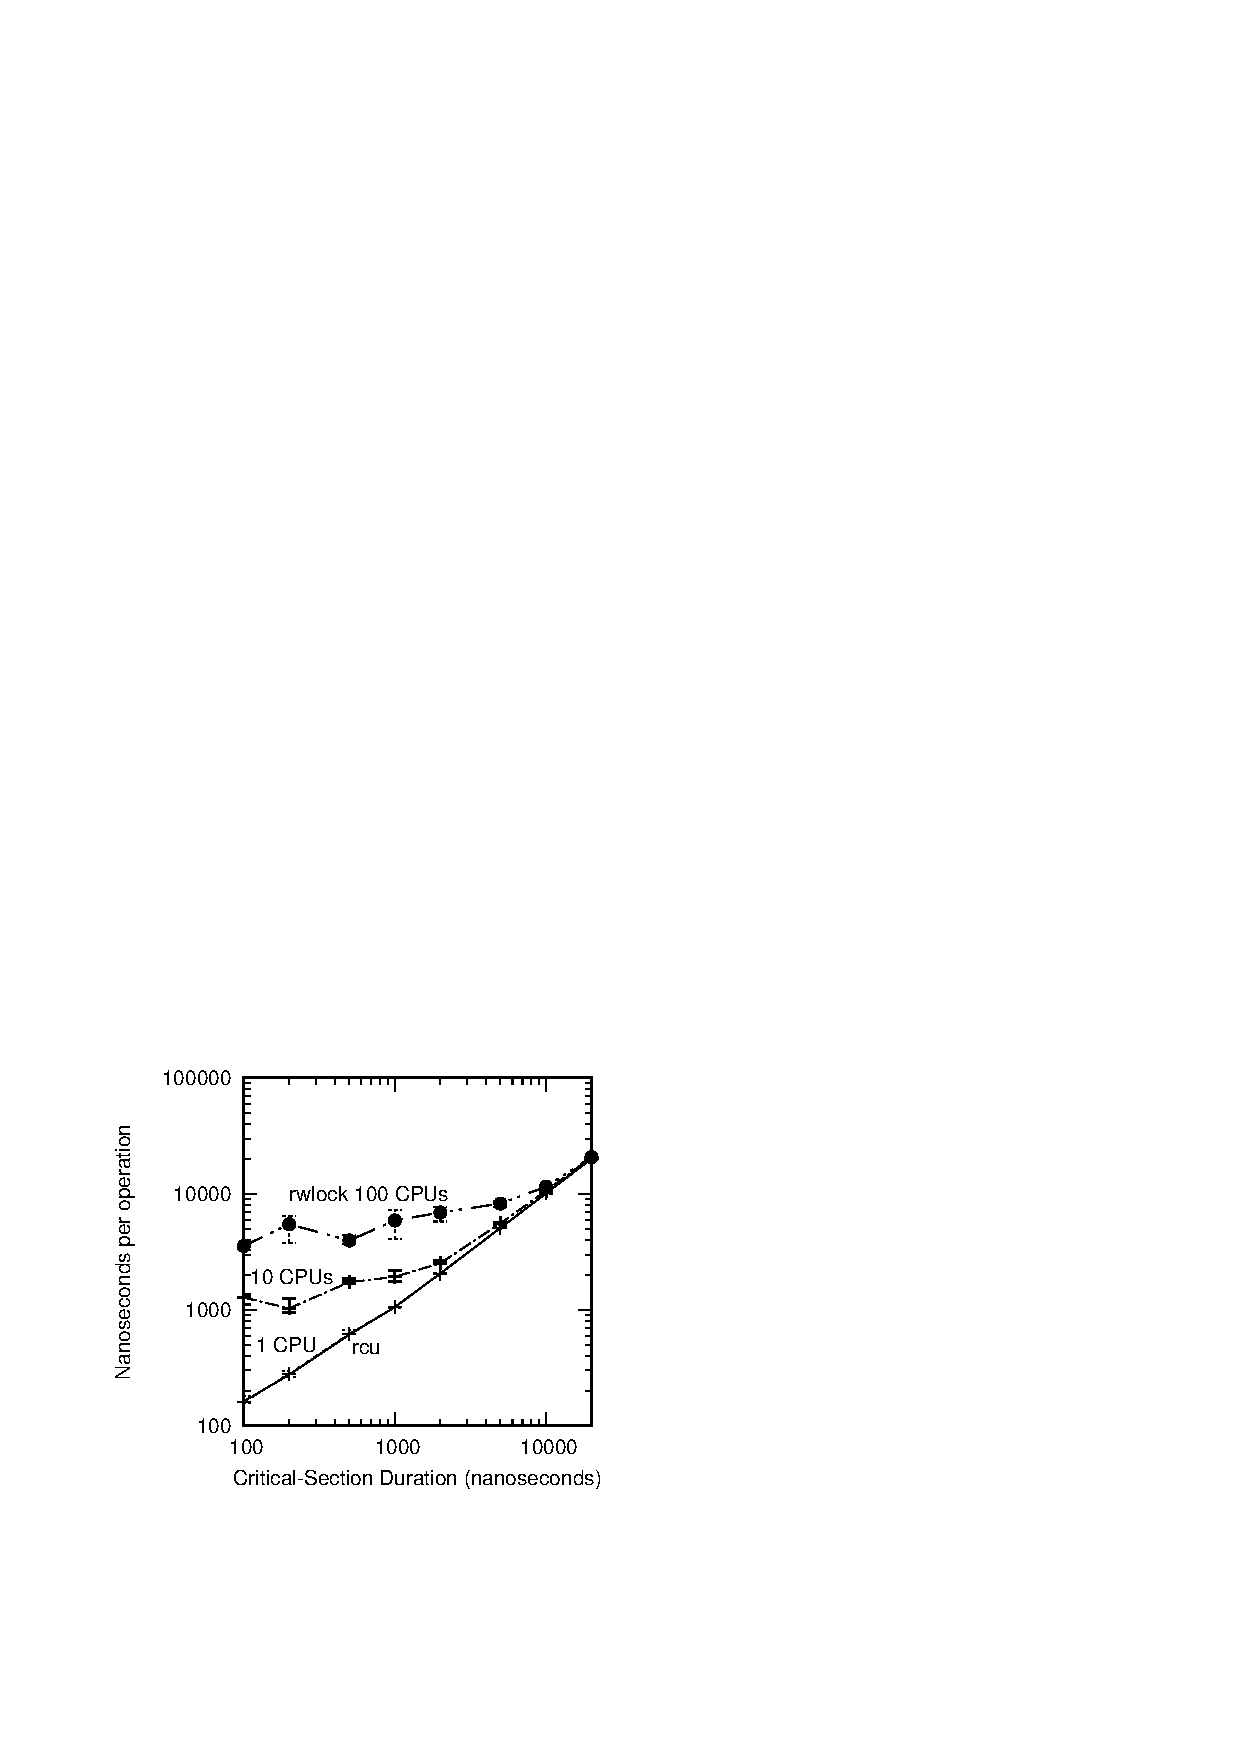
\includegraphics{defer/rwlockRCUperfwt}}
\caption{Comparison of RCU to Reader-Writer Locking as Function of Critical-Section Duration}
\label{fig:defer:Comparison of RCU to Reader-Writer Locking as Function of Critical-Section Duration}
\end{figure}

Of course, the low performance of reader-writer locking in
Figures~\ref{fig:defer:Performance Advantage of Preemptible RCU Over Reader-Writer Locking}
and~\ref{fig:defer:Performance Advantage of RCU Over Reader-Writer Locking}
is exaggerated by the unrealistic zero-length critical sections.
The performance advantages of RCU decrease as the overhead of the critical
sections increase.
This decrease can be seen in
Figure~\ref{fig:defer:Comparison of RCU to Reader-Writer Locking as Function of Critical-Section Duration},
which was run on the same system as the previous plots.
Here, the y-axis represents the sum of the overhead of the read-side
primitives and that of the critical section and the x-axis represents
the critical-section overhead in microseconds.
But please note the logscale y~axis, which means that the small
separations between the traces still represent significant differences.
This figure shows non-preemptible RCU, as can be seen by the fact that
the \co{rcu} trace drops below one nanosecond.

\QuickQuiz{
	Why aren't there error bars in
	Figure~\ref{fig:defer:Comparison of RCU to Reader-Writer Locking as Function of Critical-Section Duration}?
}\QuickQuizAnswer{
	Because for the nonzero-length critical sections, the bars
	are not much wider than the thickness of the lines.
	For the zero-length case, please refer to
	Figure~\ref{fig:defer:Performance Advantage of RCU Over Reader-Writer Locking}.
}\QuickQuizEnd

There are three traces for reader-writer locking, with the upper trace
being for 100~CPUs, the next for 10~CPUs, and the lowest for 1~CPU.
So the greater the number of CPUs and the shorter the critical sections,
the greater is RCU's performance advantage.
These performance advantages are underscored by the fact that 100-CPU
systems are no longer uncommon and that a number of system calls (and
thus any RCU read-side critical sections that they contain) complete
within a microsecond.

In addition, as is discussed in the next section,
RCU read-side primitives are almost entirely deadlock-immune.


\paragraph{Deadlock Immunity}

Although RCU offers significant performance advantages for
read-mostly workloads, one of the primary reasons for creating
RCU in the first place was in fact its immunity to read-side
deadlocks.
This immunity stems from the fact that
RCU read-side primitives do not block, spin, or even
do backwards branches, so that their execution time is deterministic.
It is therefore impossible for them to participate in a deadlock
cycle.

\QuickQuiz{
	Is there an exception to this deadlock immunity, and if so,
	what sequence of events could lead to deadlock?
}\QuickQuizAnswer{
	One way to cause a deadlock cycle involving
	RCU read-side primitives is via the following (illegal) sequence
	of statements:

\begin{VerbatimU}
rcu_read_lock();
synchronize_rcu();
rcu_read_unlock();
\end{VerbatimU}

	The \co{synchronize_rcu()} cannot return until all
	pre-existing RCU read-side critical sections complete, but
	is enclosed in an RCU read-side critical section that cannot
	complete until the \co{synchronize_rcu()} returns.
	The result is a classic self-deadlock---you get the same
	effect when attempting to write-acquire a reader-writer lock
	while read-holding it.

	Note that this self-deadlock scenario does not apply to
	RCU QSBR, because the context switch performed by the
	\co{synchronize_rcu()} would act as a quiescent state
	for this CPU, allowing a grace period to complete.
	However, this is if anything even worse, because data used
	by the RCU read-side critical section might be freed as a
	result of the grace period completing.

	In short, do not invoke synchronous RCU update-side primitives
	from within an RCU read-side critical section.
}\QuickQuizEnd

An interesting consequence of RCU's read-side deadlock immunity is
that it is possible to unconditionally upgrade an RCU
reader to an RCU updater.
Attempting to do such an upgrade with reader-writer locking results
in deadlock.
A sample code fragment that does an RCU read-to-update upgrade follows:

\begin{VerbatimN}
rcu_read_lock();
list_for_each_entry_rcu(p, &head, list_field) {
	do_something_with(p);
	if (need_update(p)) {
		spin_lock(my_lock);
		do_update(p);
		spin_unlock(&my_lock);
	}
}
rcu_read_unlock();
\end{VerbatimN}

Note that \co{do_update()} is executed under
the protection of the lock \emph{and} under RCU read-side protection.

Another interesting consequence of RCU's deadlock immunity is its
immunity to a large class of priority inversion problems.
For example, low-priority RCU readers cannot prevent a high-priority
RCU updater from acquiring the update-side lock.
Similarly, a low-priority RCU updater cannot prevent high-priority
RCU readers from entering an RCU read-side critical section.

\QuickQuiz{
	Immunity to both deadlock and priority inversion???
	Sounds too good to be true.
	Why should I believe that this is even possible?
}\QuickQuizAnswer{
	It really does work.
	After all, if it didn't work, the Linux kernel would not run.
}\QuickQuizEnd

\paragraph{Realtime Latency}

Because RCU read-side primitives neither spin nor block, they offer
excellent realtime latencies.
In addition, as noted earlier, this means that they are
immune to priority inversion
involving the RCU read-side primitives and locks.

However, RCU is susceptible to more subtle priority-inversion scenarios,
for example, a high-priority process blocked waiting for an RCU
grace period to elapse can be blocked by low-priority RCU readers
in \rt\ kernels.
This can be solved by using RCU priority
boosting~\cite{PaulEMcKenney2007BoostRCU,DinakarGuniguntala2008IBMSysJ}.

\paragraph{RCU Readers and Updaters Run Concurrently}

Because RCU readers never spin nor block, and because updaters are not
subject to any sort of rollback or abort semantics, RCU readers and
updaters must necessarily run concurrently.
This means that RCU readers might access stale data, and might even
see inconsistencies, either of which can render conversion from reader-writer
locking to RCU non-trivial.

\begin{figure}[tb]
\centering
\resizebox{3in}{!}{\includegraphics{defer/rwlockRCUupdate}}
\caption{Response Time of RCU vs. Reader-Writer Locking}
\label{fig:defer:Response Time of RCU vs. Reader-Writer Locking}
\end{figure}

However, in a surprisingly large number of situations, inconsistencies and
stale data are not problems.
The classic example is the networking routing table.
Because routing updates can take considerable time to reach a given
system (seconds or even minutes), the system will have been sending
packets the wrong way for quite some time when the update arrives.
It is usually not a problem to continue sending updates the wrong
way for a few additional milliseconds.
Furthermore, because RCU updaters can make changes without waiting for
RCU readers to finish,
the RCU readers might well see the change more quickly than would
batch-fair
reader-writer-locking readers, as shown in
Figure~\ref{fig:defer:Response Time of RCU vs. Reader-Writer Locking}.

Once the update is received, the rwlock writer cannot proceed until the
last reader completes, and subsequent readers cannot proceed until the
writer completes.
However, these subsequent readers are guaranteed to see the new value,
as indicated by the green shading of the rightmost boxes.
In contrast, RCU readers and updaters do not block each other, which permits
the RCU readers to see the updated values sooner.
Of course, because their execution overlaps that of the RCU updater,
\emph{all} of the RCU readers might well see updated values, including
the three readers that started before the update.
Nevertheless only the green-shaded rightmost RCU readers
are \emph{guaranteed} to see the updated values.

Reader-writer locking and RCU simply provide different guarantees.
With reader-writer locking, any reader that begins after the writer begins
is guaranteed to see new values, and any reader that attempts to
begin while the writer is spinning might or might not see new values,
depending on the reader/writer preference of the rwlock implementation in
question.
In contrast, with RCU, any reader that begins after the updater completes
is guaranteed to see new values, and any reader that completes after the
updater begins might or might not see new values, depending on timing.

The key point here is that, although reader-writer locking does
indeed guarantee consistency within the confines of the computer system,
there are situations where this consistency comes at the price of
increased \emph{inconsistency} with the outside world.
In other words, reader-writer locking obtains internal consistency at the
price of silently stale data with respect to the outside world.

Nevertheless, there are situations where inconsistency and stale
data within the confines of the system cannot be tolerated.
Fortunately,
there are a number of approaches that avoid inconsistency and stale
data~\cite{PaulEdwardMcKenneyPhD,Arcangeli03}, and some
methods based on reference counting are discussed in
Section~\ref{sec:defer:Reference Counting}.

\paragraph{Low-Priority RCU Readers Can Block High-Priority Reclaimers}

In Realtime RCU~\cite{DinakarGuniguntala2008IBMSysJ},
SRCU~\cite{PaulEMcKenney2006c}, or
QRCU~\cite{PaulEMcKenney2007QRCUspin} (see
Section~\ref{sec:formal:Promela Example: QRCU}),
a preempted reader will prevent
a grace period from completing, even if a high-priority task is
blocked waiting for that grace period to complete.
Realtime RCU can avoid this problem by substituting \co{call_rcu()}
for \co{synchronize_rcu()} or by using RCU priority
boosting~\cite{PaulEMcKenney2007BoostRCU,DinakarGuniguntala2008IBMSysJ},
which is still in experimental status as of early 2008.
It might become necessary to augment SRCU and QRCU with priority boosting,
but not before a clear real-world need is demonstrated.

\paragraph{RCU Grace Periods Extend for Many Milliseconds}

With the exception of QRCU and several of the ``toy'' RCU implementations
described in
Appendix~\ref{chp:app:``Toy'' RCU Implementations},
RCU grace periods extend for multiple milliseconds.
Although there are a number of techniques to render such long delays
harmless, including use of the asynchronous interfaces where available
(\co{call_rcu()} and \co{call_rcu_bh()}), this situation
is a major reason for the rule of thumb that RCU be used in read-mostly
situations.

\paragraph{Comparison of Reader-Writer Locking and RCU Code}

In the best case, the conversion from reader-writer locking to RCU
is quite simple, as shown in
Listings~\ref{lst:defer:Converting Reader-Writer Locking to RCU: Data},
\ref{lst:defer:Converting Reader-Writer Locking to RCU: Search},
and
\ref{lst:defer:Converting Reader-Writer Locking to RCU: Deletion},
all taken from
Wikipedia~\cite{WikipediaRCU}.

\begin{listing*}[htbp]
{ \scriptsize
\begin{verbbox}
 1 struct el {                           1 struct el {
 2   struct list_head lp;                2   struct list_head lp;
 3   long key;                           3   long key;
 4   spinlock_t mutex;                   4   spinlock_t mutex;
 5   int data;                           5   int data;
 6   /* Other data fields */             6   /* Other data fields */
 7 };                                    7 };
 8 DEFINE_RWLOCK(listmutex);             8 DEFINE_SPINLOCK(listmutex);
 9 LIST_HEAD(head);                      9 LIST_HEAD(head);
\end{verbbox}
}
\hspace*{0.9in}\OneColumnHSpace{-0.5in}
\theverbbox
\caption{Converting Reader-Writer Locking to RCU: Data}
\label{lst:defer:Converting Reader-Writer Locking to RCU: Data}
\end{listing*}

\begin{listing*}[htbp]
{ \scriptsize
\begin{verbbox}
 1 int search(long key, int *result)     1 int search(long key, int *result)
 2 {                                     2 {
 3   struct el *p;                       3   struct el *p;
 4                                       4
 5   read_lock(&listmutex);              5   rcu_read_lock();
 6   list_for_each_entry(p, &head, lp) { 6   list_for_each_entry_rcu(p, &head, lp) {
 7     if (p->key == key) {              7     if (p->key == key) {
 8       *result = p->data;              8       *result = p->data;
 9       read_unlock(&listmutex);        9       rcu_read_unlock();
10       return 1;                      10       return 1;
11     }                                11     }
12   }                                  12   }
13   read_unlock(&listmutex);           13   rcu_read_unlock();
14   return 0;                          14   return 0;
15 }                                    15 }
\end{verbbox}
}
\hspace*{0.9in}\OneColumnHSpace{-0.5in}
\theverbbox
\caption{Converting Reader-Writer Locking to RCU: Search}
\label{lst:defer:Converting Reader-Writer Locking to RCU: Search}
\end{listing*}

\begin{listing*}[htbp]
{ \scriptsize
\begin{verbbox}
 1 int delete(long key)                  1 int delete(long key)
 2 {                                     2 {
 3   struct el *p;                       3   struct el *p;
 4                                       4
 5   write_lock(&listmutex);             5   spin_lock(&listmutex);
 6   list_for_each_entry(p, &head, lp) { 6   list_for_each_entry(p, &head, lp) {
 7     if (p->key == key) {              7     if (p->key == key) {
 8       list_del(&p->lp);               8       list_del_rcu(&p->lp);
 9       write_unlock(&listmutex);       9       spin_unlock(&listmutex);
                                        10       synchronize_rcu();
10       kfree(p);                      11       kfree(p);
11       return 1;                      12       return 1;
12     }                                13     }
13   }                                  14   }
14   write_unlock(&listmutex);          15   spin_unlock(&listmutex);
15   return 0;                          16   return 0;
16 }                                    17 }
\end{verbbox}
}
\hspace*{0.9in}\OneColumnHSpace{-0.5in}
\theverbbox
\caption{Converting Reader-Writer Locking to RCU: Deletion}
\label{lst:defer:Converting Reader-Writer Locking to RCU: Deletion}
\end{listing*}

However, the transformation is not always this straightforward.
This is because neither the \co{spin_lock()} nor the
\co{synchronize_rcu()} in
\cref{lst:defer:Converting Reader-Writer Locking to RCU: Deletion}
exclude the readers in
\cref{lst:defer:Converting Reader-Writer Locking to RCU: Search}.
First, the \co{spin_lock()} does not interact in any way with
\co{rcu_read_lock()} and \co{rcu_read_unlock()}, thus not excluding them.
Second, although both \co{write_lock()} and \co{synchronize_rcu()}
wait for pre-existing readers, only \co{write_lock()} prevents
subsequent readers from commencing.\footnote{
	Kudos to whoever pointed this out to Paul.}
Thus, \co{synchronize_rcu()} cannot exclude readers.
It is therefore surprising that a great many situations
using reader-writer locking can be easily converted to RCU.

More-elaborate cases of replacing reader-writer locking with RCU
may be found
elsewhere~\cite{NeilBrown2015PathnameLookup,NeilBrown2015RCUwalk}.

\subsubsection{RCU is a Restricted Reference-Counting Mechanism}
\label{sec:defer:RCU is a Restricted Reference-Counting Mechanism}

Because grace periods are not allowed to complete while
there is an RCU read-side critical section in progress,
the RCU read-side primitives may be used as a restricted
reference-counting mechanism.
For example, consider the following code fragment:

\begin{VerbatimN}
rcu_read_lock();  /* acquire reference. */
p = rcu_dereference(head);
/* do something with p. */
rcu_read_unlock();  /* release reference. */
\end{VerbatimN}

The \co{rcu_read_lock()} primitive can be thought of as
acquiring a reference to \co{p}, because a grace period
starting after the \co{rcu_dereference()} assigns to \co{p}
cannot possibly end until after we reach the matching
\co{rcu_read_unlock()}.
This reference-counting scheme is restricted in that
we are not allowed to block in RCU read-side critical sections,
nor are we permitted to hand off an RCU read-side critical section
from one task to another.

Regardless of these restrictions,
the following code can safely delete \co{p}:

\begin{VerbatimN}
spin_lock(&mylock);
p = head;
rcu_assign_pointer(head, NULL);
spin_unlock(&mylock);
/* Wait for all references to be released. */
synchronize_rcu();
kfree(p);
\end{VerbatimN}

The assignment to \co{head} prevents any future references
to \co{p} from being acquired, and the \co{synchronize_rcu()}
waits for any previously acquired references to be released.

\QuickQuiz{
	But wait!
	This is exactly the same code that might be used when thinking
	of RCU as a replacement for reader-writer locking!
	What gives?
}\QuickQuizAnswer{
	This is an effect of the Law of Toy Examples:
	beyond a certain point, the code fragments look the same.
	The only difference is in how we think about the code.
	However, this difference can be extremely important.
	For but one example of the importance, consider that if we think
	of RCU as a restricted reference counting scheme, we would never
	be fooled into thinking that the updates would exclude the RCU
	read-side critical sections.

	It nevertheless is often useful to think of RCU as a replacement
	for reader-writer locking, for example, when you are replacing
	reader-writer locking with RCU.
}\QuickQuizEnd

Of course, RCU can also be combined with traditional reference counting,
as discussed in
Section~\ref{sec:together:Refurbish Reference Counting}.

\begin{figure}[tb]
\centering
\resizebox{2.5in}{!}{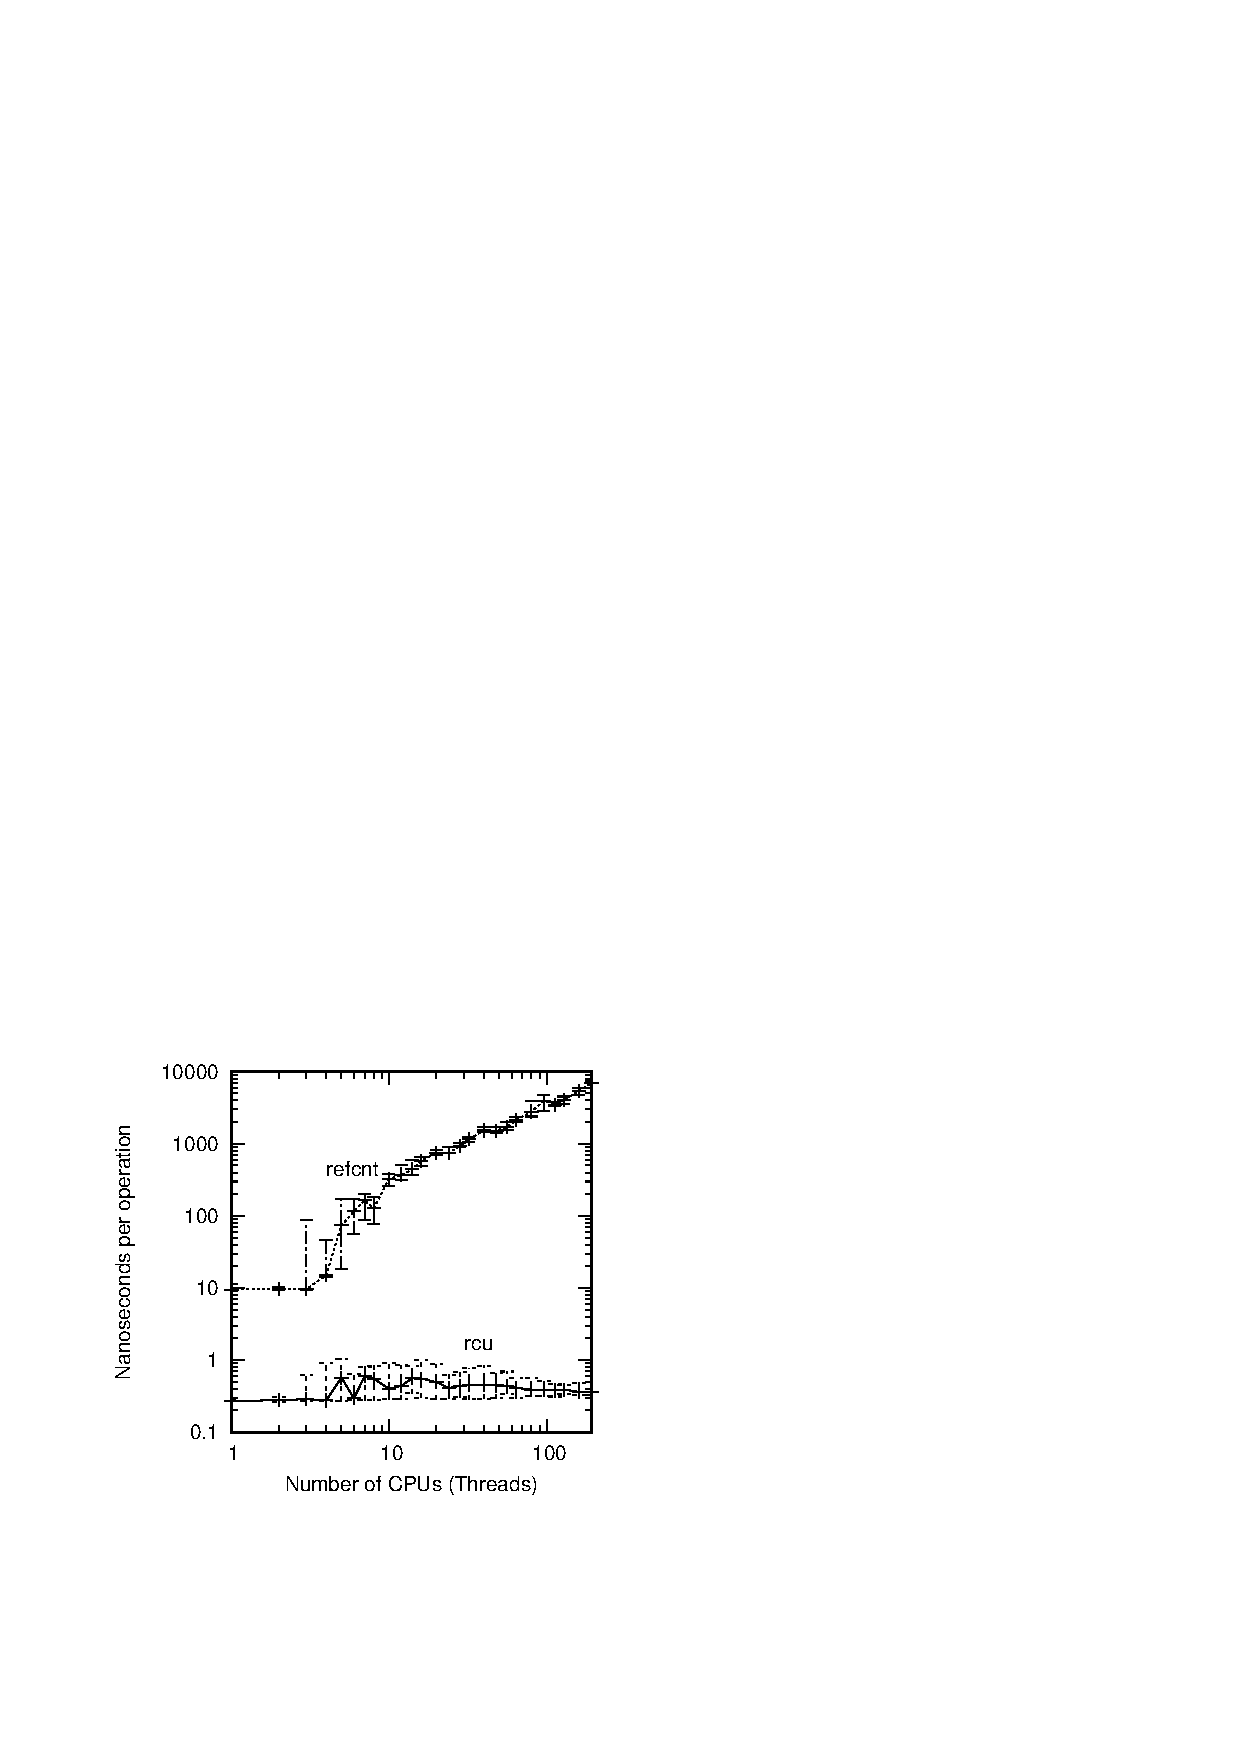
\includegraphics{defer/refcntRCUperf}}
\caption{Performance of RCU vs. Reference Counting}
\label{fig:defer:Performance of RCU vs. Reference Counting}
\end{figure}

\begin{figure}[tb]
\centering
\resizebox{2.5in}{!}{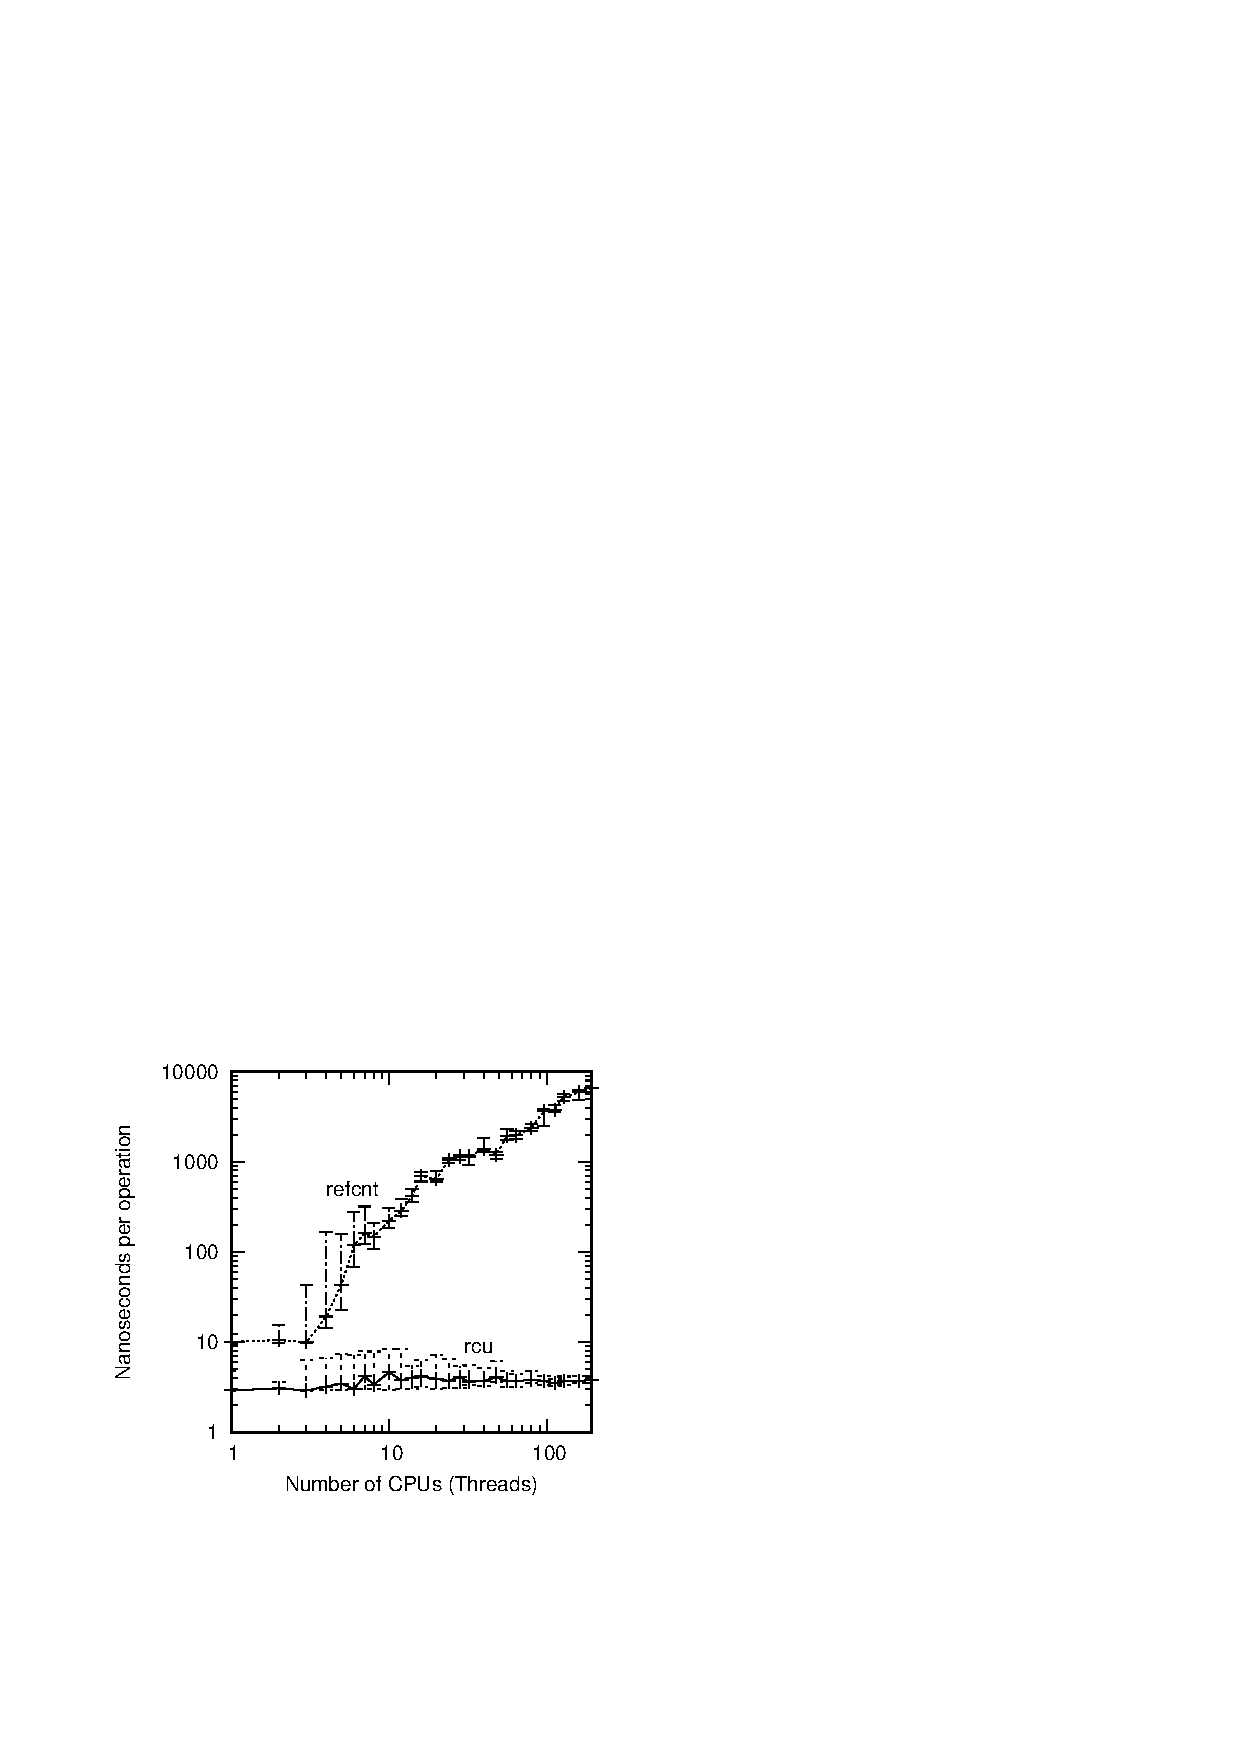
\includegraphics{defer/refRCUperfPREEMPT}}
\caption{Performance of Preemptible RCU vs. Reference Counting}
\label{fig:defer:Performance of Preemptible RCU vs. Reference Counting}
\end{figure}

But why bother?
Again, part of the answer is performance, as shown in
Figures~\ref{fig:defer:Performance of RCU vs. Reference Counting}
and~\ref{fig:defer:Performance of Preemptible RCU vs. Reference Counting},
again showing data taken on a 488-CPU 2.1\,GHz Intel x86 system
for non-preemptible and preemptible Linux-kernel RCU, respectively.
Non-preemptible RCU's advantage over reference counting ranges from
more than an order of magnitude at one CPU up to about four orders of
magnitude at 192 CPUs.
Preemptible RCU's advantage ranges from about a factor of three at
one CPU up to about three orders of magnitude at 192 CPUs.

\begin{figure}[tb]
\centering
\resizebox{2.5in}{!}{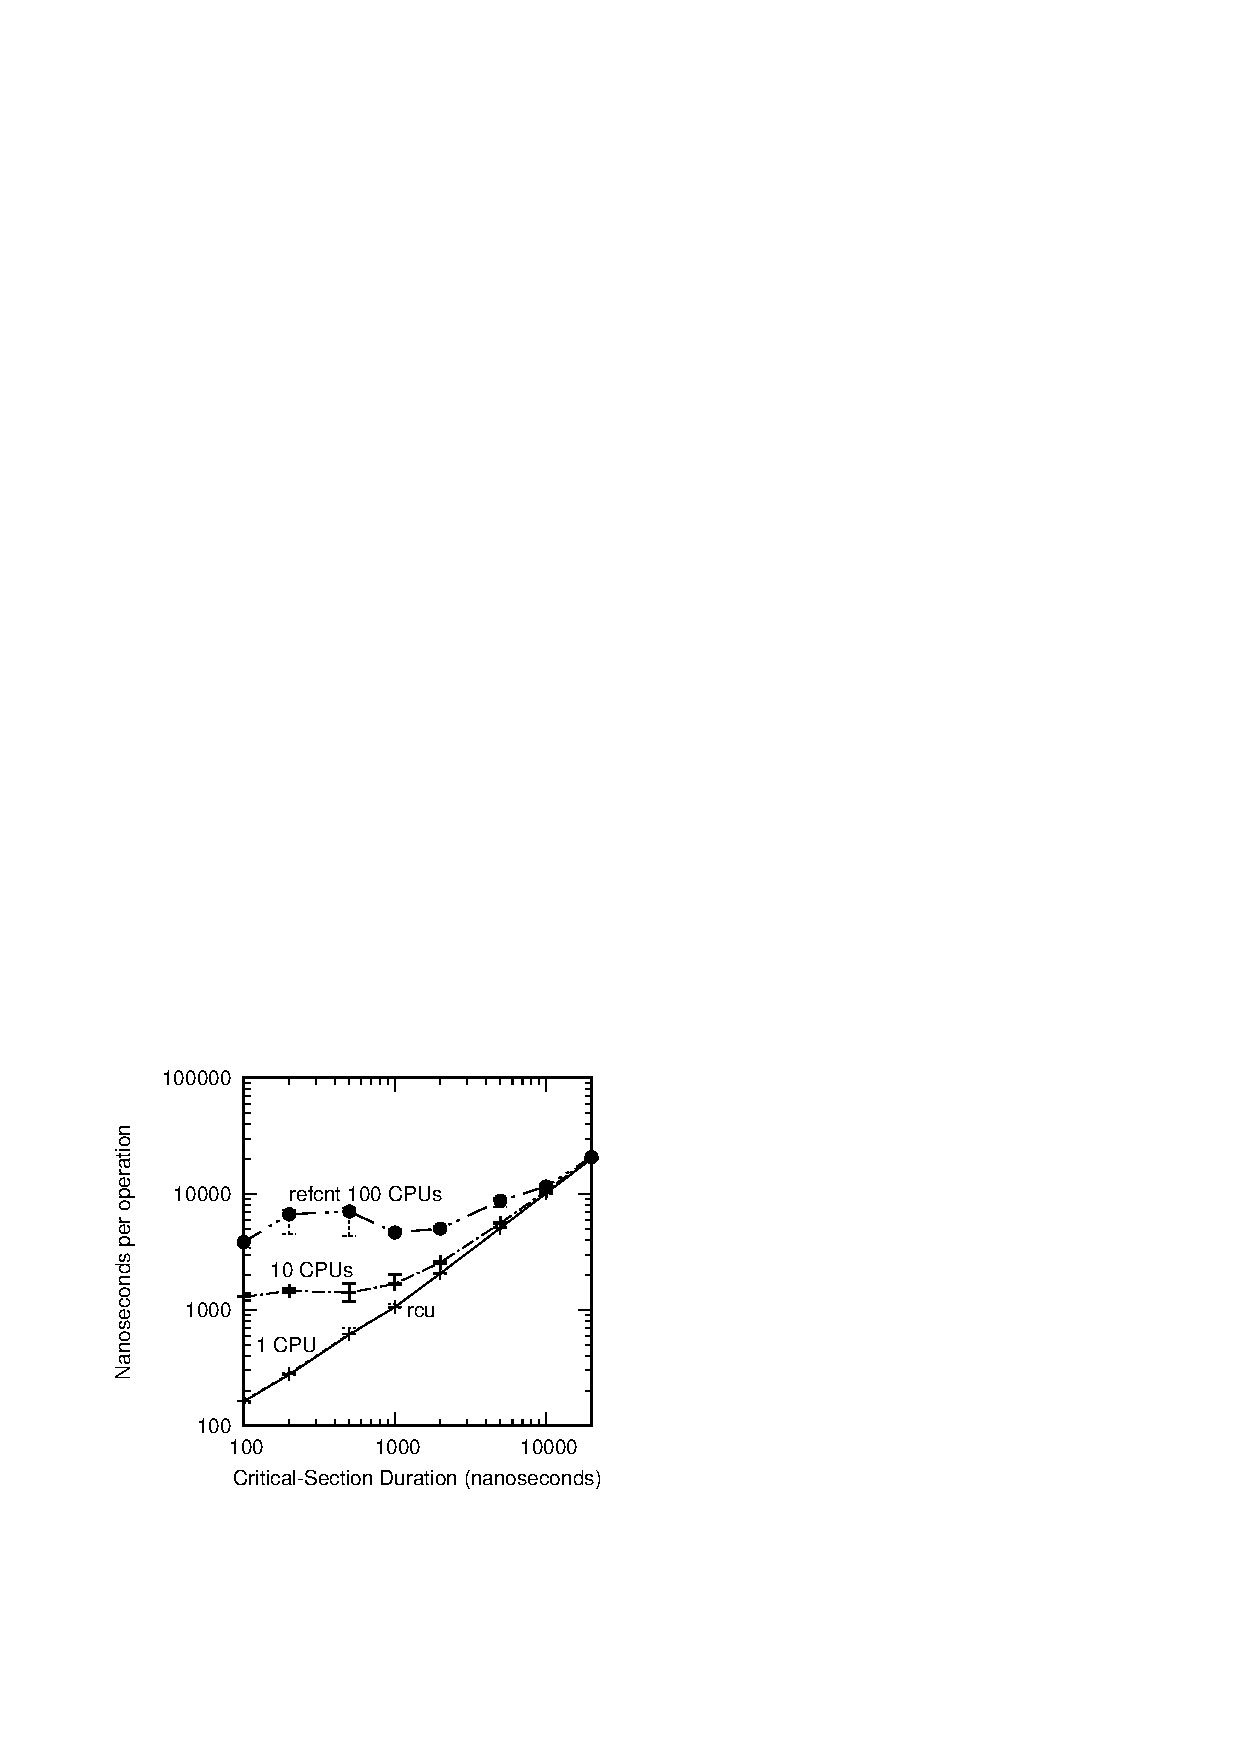
\includegraphics{defer/refRCUperfwt}}
\caption{Response Time of RCU vs. Reference Counting}
\label{fig:defer:Response Time of RCU vs. Reference Counting}
\end{figure}

However, as with reader-writer locking, the performance advantages of
RCU are most pronounced for short-duration critical sections and for
large numbers of CPUs, as shown
Figure~\ref{fig:defer:Response Time of RCU vs. Reference Counting}
for the same system.
In addition, as with reader-writer locking, many system calls (and thus
any RCU read-side critical sections that they contain) complete in
a few microseconds.

However, the restrictions that go with RCU can be quite onerous.
For example, in many cases, the prohibition against sleeping while in an RCU
read-side critical section would defeat the entire purpose.
The next section looks at ways of addressing this problem, while also
reducing the complexity of traditional reference counting, at least in
some cases.\footnote{
	Other cases might be better served by the hazard pointers
	mechanism described in \cref{sec:defer:Hazard Pointers}.}

\subsubsection{RCU is a Bulk Reference-Counting Mechanism}
\label{sec:defer:RCU is a Bulk Reference-Counting Mechanism}

As noted in the preceding section,
traditional reference counters are usually associated with a specific
data structure, or perhaps a specific group of data structures.
However, maintaining a single global reference counter for a large
variety of data structures typically results in bouncing
the cache line containing the reference count.
Such cache-line bouncing can severely degrade performance.

In contrast, RCU's lightweight read-side primitives permit
extremely frequent read-side usage with negligible performance
degradation, permitting RCU to be used as a ``bulk reference-counting''
mechanism with little or no performance penalty.
Situations where a reference must be held by a single task across a
section of code that blocks may be accommodated with
Sleepable RCU (SRCU)~\cite{PaulEMcKenney2006c}.
This fails to cover the not-uncommon situation where a reference is ``passed''
from one task to another, for example, when a reference is acquired
when starting an I/O and released in the corresponding completion
interrupt handler.
(In principle, this could be handled by the SRCU implementation,
but in practice, it is not yet clear whether this is a good tradeoff.)

Of course, SRCU brings restrictions of its own, namely that the
return value from \co{srcu_read_lock()} be passed into the
corresponding \co{srcu_read_unlock()}, and that no SRCU primitives
be invoked from hardware interrupt handlers or from non-maskable interrupt
(NMI) handlers.
The jury is still out as to how much of a problem is presented by
these restrictions, and as to how they can best be handled.

\subsubsection{RCU is a Poor Man's Garbage Collector}
\label{sec:defer:RCU is a Poor Man's Garbage Collector}

A not-uncommon exclamation made by people first learning about
RCU is ``RCU is sort of like a garbage collector!''
This exclamation has a large grain of truth, but it can also be
misleading.

Perhaps the best way to think of the relationship between RCU
and automatic garbage collectors (GCs) is that RCU resembles
a GC in that the \emph{timing} of collection is automatically
determined, but that RCU differs from a GC in that: (1) the programmer
must manually indicate when a given data structure is eligible
to be collected, and (2) the programmer must manually mark the
RCU read-side critical sections where references might legitimately
be held.

Despite these differences, the resemblance does go quite deep,
and has appeared in at least one theoretical analysis of RCU.
Furthermore, the first RCU-like mechanism I am aware of used
a garbage collector to handle the grace periods.
Nevertheless, a better way of thinking of RCU is described in the
following section.

\subsubsection{RCU Provides Existence Guarantees}
\label{sec:defer:RCU Provides Existence Guarantees}

Gamsa et al.~\cite{Gamsa99}
discuss existence guarantees and describe how a mechanism
resembling RCU can be used to provide these existence guarantees
(see section~5 on page 7 of the PDF), and
Section~\ref{sec:locking:Lock-Based Existence Guarantees}
discusses how to guarantee existence via locking, along with the
ensuing disadvantages of doing so.
The effect is that if any RCU-protected data element is accessed
within an RCU read-side critical section, that data element is
guaranteed to remain in existence for the duration of that RCU
read-side critical section.

\begin{listing}[tbp]
\begin{fcvlabel}[ln:defer:Existence Guarantees Enable Per-Element Locking]
\begin{VerbatimL}[commandchars=\\\@\$]
int delete(int key)
{
	struct element *p;
	int b;

	b = hashfunction(key);			\lnlbl@hash$
	rcu_read_lock();			\lnlbl@rdlock$
	p = rcu_dereference(hashtable[b]);
	if (p == NULL || p->key != key) {	\lnlbl@chkkey$
		rcu_read_unlock();		\lnlbl@rdunlock1$
		return 0;			\lnlbl@ret_0:a$
	}
	spin_lock(&p->lock);			\lnlbl@acq$
	if (hashtable[b] == p && p->key == key) {\lnlbl@chkkey2$
		rcu_read_unlock();		\lnlbl@rdunlock2$
		rcu_assign_pointer(hashtable[b], NULL);\lnlbl@remove$
		spin_unlock(&p->lock);		\lnlbl@rel1$
		synchronize_rcu();		\lnlbl@sync_rcu$
		kfree(p);			\lnlbl@kfree$
		return 1;			\lnlbl@ret_1$
	}
	spin_unlock(&p->lock);			\lnlbl@rel2$
	rcu_read_unlock();			\lnlbl@rdunlock3$
	return 0;				\lnlbl@ret_0:b$
}
\end{VerbatimL}
\end{fcvlabel}
\caption{Existence Guarantees Enable Per-Element Locking}
\label{lst:defer:Existence Guarantees Enable Per-Element Locking}
\end{listing}

\begin{fcvref}[ln:defer:Existence Guarantees Enable Per-Element Locking]
Listing~\ref{lst:defer:Existence Guarantees Enable Per-Element Locking}
demonstrates how RCU-based existence guarantees can enable
per-element locking via a function that deletes an element from
a hash table.
Line~\lnref{hash} computes a hash function, and line~\lnref{rdlock} enters an RCU
read-side critical section.
If line~\lnref{chkkey} finds that the corresponding bucket of the hash table is
empty or that the element present is not the one we wish to delete,
then line~\lnref{rdunlock1} exits the RCU read-side critical section and
line~\lnref{ret_0:a}
indicates failure.
\end{fcvref}

\QuickQuiz{
	What if the element we need to delete is not the first element
	of the list on
        line~\ref{ln:defer:Existence Guarantees Enable Per-Element Locking:chkkey} of
	Listing~\ref{lst:defer:Existence Guarantees Enable Per-Element Locking}?
}\QuickQuizAnswer{
	As with
	Listing~\ref{lst:locking:Per-Element Locking Without Existence Guarantees},
	this is a very simple hash table with no chaining, so the only
	element in a given bucket is the first element.
	The reader is again invited to adapt this example to a hash table with
	full chaining.
}\QuickQuizEnd

\begin{fcvref}[ln:defer:Existence Guarantees Enable Per-Element Locking]
Otherwise, line~\lnref{acq} acquires the update-side spinlock, and
line~\lnref{chkkey2} then checks that the element is still the one that we want.
If so, line~\lnref{rdunlock2} leaves the RCU read-side critical section,
line~\lnref{remove} removes it from the table, line~\lnref{rel1} releases
the lock, line~\lnref{sync_rcu} waits for all pre-existing RCU read-side critical
sections to complete, line~\lnref{kfree} frees the newly removed element,
and line~\lnref{ret_1} indicates success.
If the element is no longer the one we want, line~\lnref{rel2} releases
the lock, line~\lnref{rdunlock3} leaves the RCU read-side critical section,
and line~\lnref{ret_0:b} indicates failure to delete the specified key.
\end{fcvref}

\QuickQuizSeries{%
\QuickQuizB{
	\begin{fcvref}[ln:defer:Existence Guarantees Enable Per-Element Locking]
	Why is it OK to exit the RCU read-side critical section on
	line~\lnref{rdunlock2} of
	Listing~\ref{lst:defer:Existence Guarantees Enable Per-Element Locking}
	before releasing the lock on line~\lnref{rel1}?
	\end{fcvref}
}\QuickQuizAnswerB{
	\begin{fcvref}[ln:defer:Existence Guarantees Enable Per-Element Locking]
	First, please note that the second check on line~\lnref{chkkey2} is
	necessary because some other
	CPU might have removed this element while we were waiting
	to acquire the lock.
	However, the fact that we were in an RCU read-side critical section
	while acquiring the lock guarantees that this element could not
	possibly have been re-allocated and re-inserted into this
	hash table.
	Furthermore, once we acquire the lock, the lock itself guarantees
	the element's existence, so we no longer need to be in an
	RCU read-side critical section.

	The question as to whether it is necessary to re-check the
	element's key is left as an exercise to the reader.
	% A re-check is necessary if the key can mutate or if it is
	% necessary to reject deleted entries (in cases where deletion
	% is recorded by mutating the key.
	\end{fcvref}
}\QuickQuizEndB
%
\QuickQuizE{
	\begin{fcvref}[ln:defer:Existence Guarantees Enable Per-Element Locking]
	Why not exit the RCU read-side critical section on
	line~\lnref{rdunlock3} of
	Listing~\ref{lst:defer:Existence Guarantees Enable Per-Element Locking}
	before releasing the lock on line~\lnref{rel2}?
	\end{fcvref}
}\QuickQuizAnswerE{
	Suppose we reverse the order of these two lines.
	Then this code is vulnerable to the following sequence of
	events:
	\begin{enumerate}
	\begin{fcvref}[ln:defer:Existence Guarantees Enable Per-Element Locking]
	\item	CPU~0 invokes \co{delete()}, and finds the element
		to be deleted, executing through line~\lnref{rdunlock2}.
		It has not yet actually deleted the element, but
		is about to do so.
	\item	CPU~1 concurrently invokes \co{delete()}, attempting
		to delete this same element.
		However, CPU~0 still holds the lock, so CPU~1 waits
		for it at line~\lnref{acq}.
	\item	CPU~0 executes lines~\lnref{remove} and~\lnref{rel1},
		and blocks at line~\lnref{sync_rcu} waiting for CPU~1
		to exit its RCU read-side critical section.
	\item	CPU~1 now acquires the lock, but the test on line~\lnref{chkkey2}
		fails because CPU~0 has already removed the element.
		CPU~1 now executes line~\lnref{rel2}
                (which we switched with line~\lnref{rdunlock3}
		for the purposes of this Quick Quiz)
		and exits its RCU read-side critical section.
	\item	CPU~0 can now return from \co{synchronize_rcu()},
		and thus executes line~\lnref{kfree}, sending the element to
		the freelist.
	\item	CPU~1 now attempts to release a lock for an element
		that has been freed, and, worse yet, possibly
		reallocated as some other type of data structure.
		This is a fatal memory-corruption error.
	\end{fcvref}
	\end{enumerate}
}\QuickQuizEndE
}

Alert readers will recognize this as only a slight variation on
the original ``RCU is a way of waiting for things to finish'' theme,
which is addressed in
Section~\ref{sec:defer:RCU is a Way of Waiting for Things to Finish}.
They might also note the deadlock-immunity advantages over the lock-based
existence guarantees discussed in
Section~\ref{sec:locking:Lock-Based Existence Guarantees}.

\subsubsection{RCU is a Way of Providing Type-Safe Memory}
\label{sec:defer:RCU is a Way of Providing Type-Safe Memory}

A number of lockless algorithms do not require that a given data
element keep the same identity through a given RCU read-side critical
section referencing it---but only if that data element retains the
same type.
In other words, these lockless algorithms can tolerate a given data
element being freed and reallocated as the same type of structure
while they are referencing it, but must prohibit a change in type.
This guarantee, called ``type-safe memory'' in
academic literature~\cite{Cheriton96a},
is weaker than the existence guarantees in the
previous section, and is therefore quite a bit harder to work with.
Type-safe memory algorithms in the Linux kernel make use of slab caches,
specially marking these caches with \co{SLAB_TYPESAFE_BY_RCU}
so that RCU is used when returning a freed-up
slab to system memory.
This use of RCU guarantees that any in-use element of
such a slab will remain in that slab, thus retaining its type,
for the duration of any pre-existing RCU read-side critical sections.

\QuickQuiz{
	But what if there is an arbitrarily long series of RCU
	read-side critical sections in multiple threads, so that at
	any point in time there is at least one thread in the system
	executing in an RCU read-side critical section?
	Wouldn't that prevent any data from a \co{SLAB_TYPESAFE_BY_RCU}
	slab ever being returned to the system, possibly resulting
	in OOM events?
}\QuickQuizAnswer{
	There could certainly be an arbitrarily long period of time
	during which at least one thread is always in an RCU read-side
	critical section.
	However, the key words in the description in
	Section~\ref{sec:defer:RCU is a Way of Providing Type-Safe Memory}
	are ``in-use'' and ``pre-existing''.
	Keep in mind that a given RCU read-side critical section is
	conceptually only permitted to gain references to data elements
	that were in use at the beginning of that critical section.
	Furthermore, remember that a slab cannot be returned to the
	system until all of its data elements have been freed, in fact,
	the RCU grace period cannot start until after they have all been
	freed.

	Therefore, the slab cache need only wait for those RCU read-side
	critical sections that started before the freeing of the last element
	of the slab.
	This in turn means that any RCU grace period that begins after
	the freeing of the last element will do---the slab may be returned
	to the system after that grace period ends.
}\QuickQuizEnd

These algorithms typically use a validation step that checks to make
sure that the newly referenced data structure really is the one that
was requested~\cite[Section 2.5]{LaninShasha1986TSM}.
These validation checks require that portions of the data structure
remain untouched by the free-reallocate process.
Such validation checks are usually very hard to get right, and can
hide subtle and difficult bugs.

Therefore, although type-safety-based lockless algorithms can be extremely
helpful in a very few difficult situations, you should instead use existence
guarantees where possible.
Simpler is after all almost always better!

\subsubsection{RCU is a Way of Waiting for Things to Finish}
\label{sec:defer:RCU is a Way of Waiting for Things to Finish}

As noted in Section~\ref{sec:defer:RCU Fundamentals}
an important component
of RCU is a way of waiting for RCU readers to finish.
One of
RCU's great strength is that it allows you to wait for each of
thousands of different things to finish without having to explicitly
track each and every one of them, and without having to worry about
the performance degradation, scalability limitations, complex deadlock
scenarios, and memory-leak hazards that are inherent in schemes that
use explicit tracking.

In this section, we will show how \co{synchronize_sched()}'s
read-side counterparts (which include anything that disables preemption,
along with hardware operations and
primitives that disable interrupts) permit you to implement interactions with
non-maskable interrupt
(NMI) handlers that would be quite difficult if using locking.
This approach has been called ``Pure RCU''~\cite{PaulEdwardMcKenneyPhD},
and it is used in a number of places in the Linux kernel.

The basic form of such ``Pure RCU'' designs is as follows:

\begin{enumerate}
\item	Make a change, for example, to the way that the OS reacts to an NMI.
\item	Wait for all pre-existing read-side critical sections to
	completely finish (for example, by using the
	\co{synchronize_sched()} primitive).
	The key observation here is that subsequent RCU read-side critical
	sections are guaranteed to see whatever change was made.
\item	Clean up, for example, return status indicating that the
	change was successfully made.
\end{enumerate}

The remainder of this section presents example code adapted from
the Linux kernel.
In this example, the \co{timer_stop} function uses
\co{synchronize_sched()} to ensure that all in-flight NMI
notifications have completed before freeing the associated resources.
A simplified version of this code is shown
Listing~\ref{lst:defer:Using RCU to Wait for NMIs to Finish}.

\begin{listing}[tbp]
\begin{fcvlabel}[ln:defer:Using RCU to Wait for NMIs to Finish]
\begin{VerbatimL}[commandchars=\\\@\$]
struct profile_buffer {				\lnlbl@struct:b$
	long size;
	atomic_t entry[0];
};						\lnlbl@struct:e$
static struct profile_buffer *buf = NULL;	\lnlbl@struct:buf$

void nmi_profile(unsigned long pcvalue)		\lnlbl@nmi_profile:b$
{
	struct profile_buffer *p = rcu_dereference(buf);\lnlbl@nmi_profile:rcu_deref$

	if (p == NULL)				\lnlbl@nmi_profile:if_NULL$
		return;				\lnlbl@nmi_profile:ret:a$
	if (pcvalue >= p->size)			\lnlbl@nmi_profile:if_oor$
		return;				\lnlbl@nmi_profile:ret:b$
	atomic_inc(&p->entry[pcvalue]);		\lnlbl@nmi_profile:inc$
}						\lnlbl@nmi_profile:e$

void nmi_stop(void)				\lnlbl@nmi_stop:b$
{
	struct profile_buffer *p = buf;		\lnlbl@nmi_stop:fetch$

	if (p == NULL)				\lnlbl@nmi_stop:if_NULL$
		return;				\lnlbl@nmi_stop:ret$
	rcu_assign_pointer(buf, NULL);		\lnlbl@nmi_stop:NULL$
	synchronize_sched();			\lnlbl@nmi_stop:sync_sched$
	kfree(p);				\lnlbl@nmi_stop:kfree$
}						\lnlbl@nmi_stop:e$
\end{VerbatimL}
\end{fcvlabel}
\caption{Using RCU to Wait for NMIs to Finish}
\label{lst:defer:Using RCU to Wait for NMIs to Finish}
\end{listing}

\begin{fcvref}[ln:defer:Using RCU to Wait for NMIs to Finish:struct]
\Clnrefrange{b}{e} define a \co{profile_buffer} structure, containing a
size and an indefinite array of entries.
Line~\lnref{buf} defines a pointer to a profile buffer, which is
presumably initialized elsewhere to point to a dynamically allocated
region of memory.
\end{fcvref}

\begin{fcvref}[ln:defer:Using RCU to Wait for NMIs to Finish:nmi_profile]
\Clnrefrange{b}{e} define the \co{nmi_profile()} function,
which is called from within an NMI handler.
As such, it cannot be preempted, nor can it be interrupted by a normal
interrupts handler, however, it is still subject to delays due to cache misses,
ECC errors, and cycle stealing by other hardware threads within the same
core.
Line~\lnref{rcu_deref} gets a local pointer to the profile buffer using the
\co{rcu_dereference()} primitive to ensure memory ordering on
DEC Alpha, and
lines~\lnref{if_NULL} and~\lnref{ret:a} exit from this function if there is no
profile buffer currently allocated, while lines~\lnref{if_oor} and~\lnref{ret:b}
exit from this function if the \co{pcvalue} argument
is out of range.
Otherwise, line~\lnref{inc} increments the profile-buffer entry indexed
by the \co{pcvalue} argument.
Note that storing the size with the buffer guarantees that the
range check matches the buffer, even if a large buffer is suddenly
replaced by a smaller one.
\end{fcvref}

\begin{fcvref}[ln:defer:Using RCU to Wait for NMIs to Finish:nmi_stop]
\Clnrefrange{b}{e} define the \co{nmi_stop()} function,
where the caller is responsible for mutual exclusion (for example,
holding the correct lock).
Line~\lnref{fetch} fetches a pointer to the profile buffer, and
lines~\lnref{if_NULL} and~\lnref{ret} exit the function if there is no buffer.
Otherwise, line~\lnref{NULL} \co{NULL}s out the profile-buffer pointer
(using the \co{rcu_assign_pointer()} primitive to maintain
memory ordering on weakly ordered machines),
and line~\lnref{sync_sched} waits for an RCU Sched grace period to elapse,
in particular, waiting for all non-preemptible regions of code,
including NMI handlers, to complete.
Once execution continues at line~\lnref{kfree}, we are guaranteed that
any instance of \co{nmi_profile()} that obtained a
pointer to the old buffer has returned.
It is therefore safe to free the buffer, in this case using the
\co{kfree()} primitive.
\end{fcvref}

\QuickQuiz{
	Suppose that the \co{nmi_profile()} function was preemptible.
	What would need to change to make this example work correctly?
}\QuickQuizAnswer{
	One approach would be to use
	\co{rcu_read_lock()} and \co{rcu_read_unlock()}
	in \co{nmi_profile()}, and to replace the
	\co{synchronize_sched()} with \co{synchronize_rcu()},
	perhaps as shown in
	Listing~\ref{lst:defer:Using RCU to Wait for Mythical Preemptible NMIs to Finish}.
%
\begin{listing}[tb]
\begin{VerbatimL}
struct profile_buffer {
	long size;
	atomic_t entry[0];
};
static struct profile_buffer *buf = NULL;

void nmi_profile(unsigned long pcvalue)
{
	struct profile_buffer *p;

	rcu_read_lock();
	p = rcu_dereference(buf);
	if (p == NULL) {
		rcu_read_unlock();
		return;
	}
	if (pcvalue >= p->size) {
		rcu_read_unlock();
		return;
	}
	atomic_inc(&p->entry[pcvalue]);
	rcu_read_unlock();
}

void nmi_stop(void)
{
	struct profile_buffer *p = buf;

	if (p == NULL)
		return;
	rcu_assign_pointer(buf, NULL);
	synchronize_rcu();
	kfree(p);
}
\end{VerbatimL}
\caption{Using RCU to Wait for Mythical Preemptible NMIs to Finish}
\label{lst:defer:Using RCU to Wait for Mythical Preemptible NMIs to Finish}
\end{listing}
%
}\QuickQuizEnd

In short, RCU makes it easy to dynamically switch among profile
buffers (you just \emph{try} doing this efficiently with atomic
operations, or at all with locking!).
However, RCU is normally used at a higher level of abstraction, as
was shown in the previous sections.

\subsubsection{RCU Usage Summary}
\label{sec:defer:RCU Usage Summary}

At its core, RCU is nothing more nor less than an API that provides:

\begin{enumerate}
\item	a publish-subscribe mechanism for adding new data,
\item	a way of waiting for pre-existing RCU readers to finish, and
\item	a discipline of maintaining multiple versions to permit change
	without harming or unduly delaying concurrent RCU readers.
\end{enumerate}

That said, it is possible to build higher-level constructs
on top of RCU, including the reader-writer-locking, reference-counting,
and existence-guarantee constructs listed in the earlier sections.
Furthermore, I have no doubt that the Linux community will continue to
find interesting new uses for RCU,
as well as for any of a number of other synchronization primitives.

\begin{figure}[tbh]
\centering
\resizebox{3in}{!}{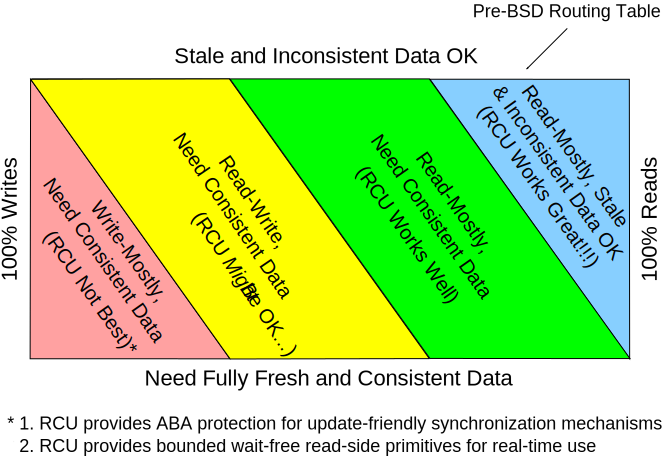
\includegraphics{defer/RCUApplicability}}
\caption{RCU Areas of Applicability}
\label{fig:defer:RCU Areas of Applicability}
\end{figure}

In the meantime,
Figure~\ref{fig:defer:RCU Areas of Applicability}
shows some rough rules of thumb on where RCU is most helpful.

As shown in the blue box at the top of the figure, RCU works best if
you have read-mostly data where stale and inconsistent
data is permissible (but see below for more information on stale and
inconsistent data).
The canonical example of this case in the Linux kernel is routing tables.
Because it may have taken many seconds or even minutes for the
routing updates to propagate across the Internet, the system
has been sending packets the wrong way for quite some time.
Having some small probability of continuing to send some of them the wrong
way for a few more milliseconds is almost never a problem.

If you have a read-mostly workload where consistent data is required,
RCU works well, as shown by the green ``read-mostly, need consistent data''
box.
One example of this case is the Linux kernel's mapping from user-level
System-V semaphore IDs to the corresponding in-kernel data structures.
Semaphores tend to be used far more frequently than they are created
and destroyed, so this mapping is read-mostly.
However, it would be erroneous to perform a semaphore operation on
a semaphore that has already been deleted.
This need for consistency is handled by using the lock in the
in-kernel semaphore data structure, along with a ``deleted''
flag that is set when deleting a semaphore.
If a user ID maps to an in-kernel data structure with the
``deleted'' flag set, the data structure is ignored, so that
the user ID is flagged as invalid.

Although this requires that the readers acquire a lock for the
data structure representing the semaphore itself,
it allows them to dispense with locking for the
mapping data structure.
The readers therefore locklessly
traverse the tree used to map from ID to data structure,
which in turn greatly improves performance, scalability, and
real-time response.

As indicated by the yellow ``read-write'' box, RCU can also be useful
for read-write
workloads where consistent data is required, although usually in
conjunction with a number of other synchronization primitives.
For example, the directory-entry cache in recent Linux kernels uses RCU in
conjunction with sequence locks, per-CPU locks, and per-data-structure
locks to allow lockless traversal of pathnames in the common case.
Although RCU can be very beneficial in this read-write case, such
use is often more complex than that of the read-mostly cases.

Finally, as indicated by the red box at the bottom of the figure,
update-mostly workloads requiring
consistent data are rarely good places to use RCU, though there are some
exceptions~\cite{MathieuDesnoyers2012URCU}.
In addition, as noted in
Section~\ref{sec:defer:RCU is a Way of Providing Type-Safe Memory},
within the Linux kernel, the \co{SLAB_TYPESAFE_BY_RCU}
slab-allocator flag provides type-safe memory to RCU readers, which can
greatly simplify non-blocking synchronization and other lockless
algorithms.

In short, RCU is an API that includes a publish-subscribe mechanism for
adding new data, a way of waiting for pre-existing RCU readers to finish,
and a discipline of maintaining multiple versions to allow updates to
avoid harming or unduly delaying concurrent RCU readers.
This RCU API is best suited for read-mostly situations, especially if
stale and inconsistent data can be tolerated by the application.
